\chapter{Methods}
The proposed processing techniques and methods used for evaluating finger movements and recognizing errors requires six steps:  (1) removal of artifacts from \ac{EMG} data, (2) segmentation of the \ac{EMG} data into individual movements, (3) division of the \ac{EMG} data into 11 folds (11 is the number of the features we are preprocessing the EMG data with), (4) windowing, (5) feature extraction, (6) classification. The machine learning model learns the patterns of the preprocessed data by the selected features, segmented individual finger movements. Based on the detection accuracies of each machine learning model, allows us to have feedback on which of the features are working best on the \ac{EMG} data.\\
\section{Pipeline summary}
In Fig. \ref{fig:pipeline_summary} the overview of the system's pipeline is depicted. \\
\begin{figure}[h!]
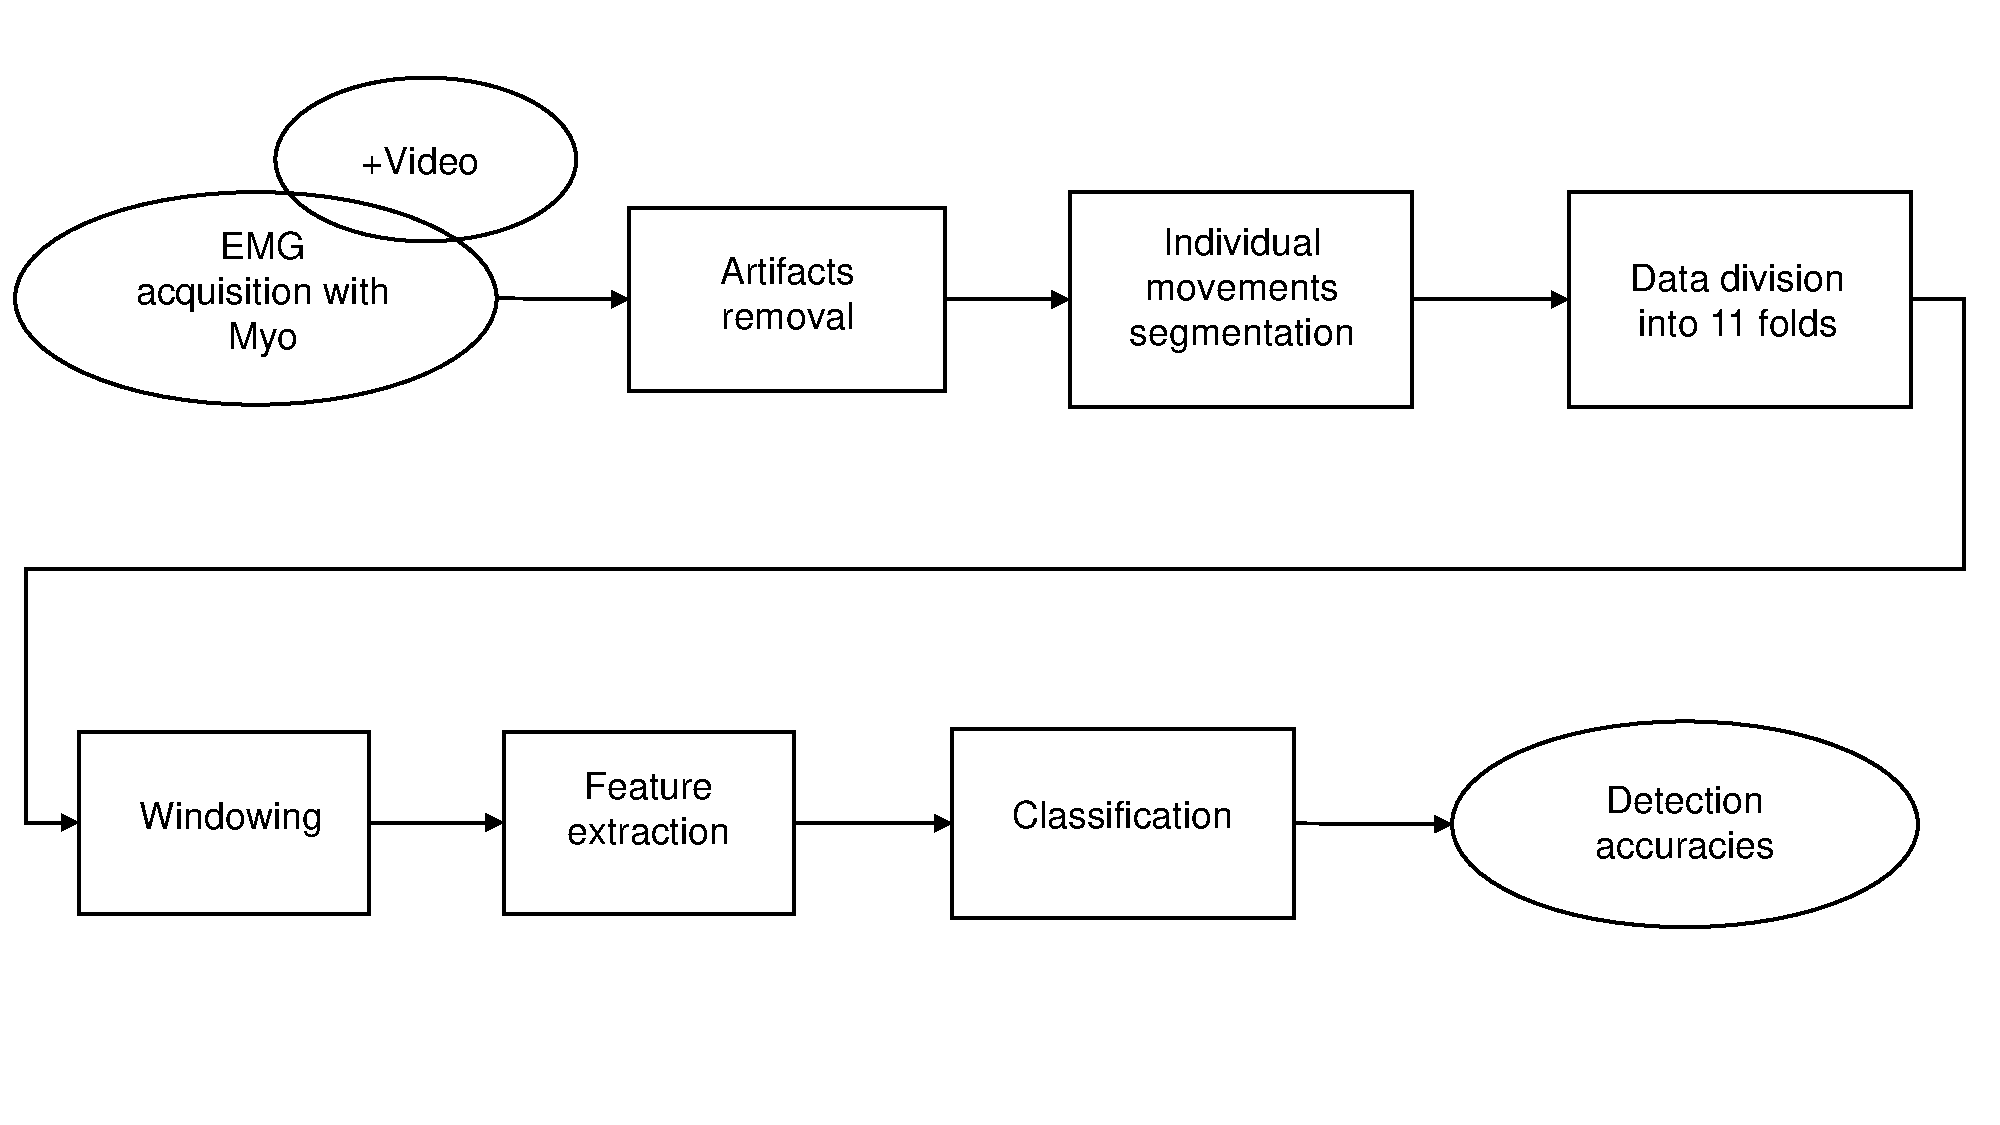
\includegraphics[width=15cm,left,keepaspectratio]{figures/pipeline_summary.pdf}
\caption{Overview of the pipeline}
\label{fig:pipeline_summary}
\end{figure}
\section{Data collection}
In Fig. \ref{fig:data_collection} we can see how the data are acquired. Firstly, the subject wears the Myo armband in his/her arm and via Bluetooth connection the Myo armband is connected with a mobile phone. After the completion of the corresponding finger gesture the zip folder with the acquired signals and the video recording are uploaded to the cloud. The \ac{EMG} signals and the video recordings are downloaded to the PC. The video recording is used next, in order to determine the intervals of the gestures we are interested in. Then, we input the frames of interest in the Cutter App, an application implemented by Seiffarth Johannes, and the \ac{EMG} signals are segmented in the corresponding frame intervals. Also, with the same application we can visualize the \ac{EMG} waveforms of the different recordings and to remove any artifacts. In the current work, due to the variable frame rate of the cell phone's camera the frames of the video did not correspond to the corresponding waveform in time, thus leading to artifacts. This behavior of the mobile device's camera happened unexpectedly during the different takes. Therefore, every recording was examined carefully before segmenting it.
\begin{figure}[h!]
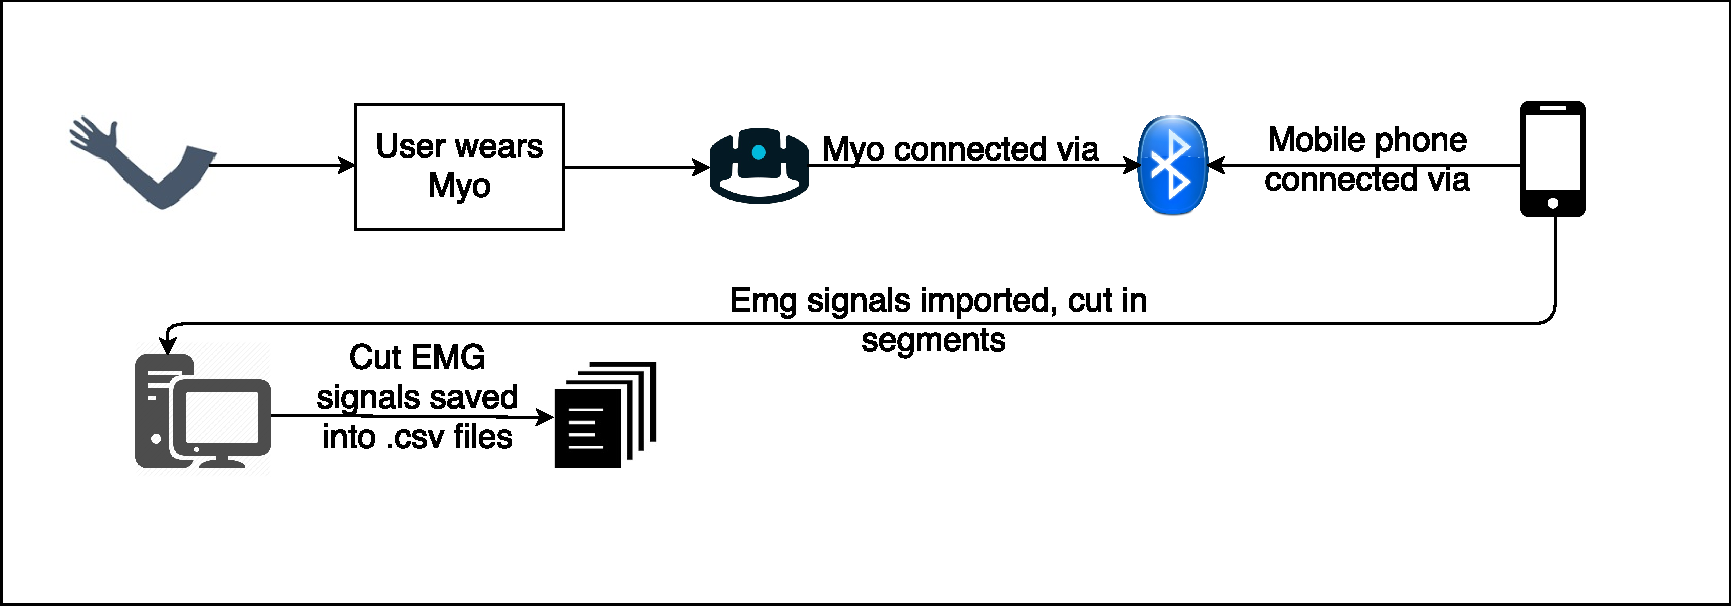
\includegraphics[width=15cm,left,keepaspectratio]{figures/data_collection}
\caption{Data collection}
\label{fig:data_collection}
\end{figure}
\section{Cross-Validation}
Next, as the Fig. \ref{fig:division_into_5_folds} demonstrates, the data are divided into training, testing and evaluation folders. Specifically, we start by removing 20\% of the segmented data and we create a evaluation folder with this data. Until the machine learning model is fully developed we do not touch the data from the evaluation folder. In addition, cross validation technique allows to compensate for small data sets and makes our results more robust. Then, we have to decide on the number of the folds. If we choose a large number of folds we will have too little data in each fold and if we choose a small number of folds, the method will not be serving its purpose. In our case, we choose to create five training and test folds and one evaluation folder. The remaining 80\% of the data, will be our train and test data.\\
After the creation of the evaluation folder, we create the five test folders by dividing randomly the remaining data accordingly to the number of the folders we created. In our case, we take a random 20\% from the remaining data and distribute it to each of the five test folders. Then, we create each of the five train folders by combining all the data from the test folders but excluding the folder with the mutual shared number. For example, the train folder with the number one will take all the data from the test folders with the number two, three, four and five thus, excluding the test folder with the number one. This applies for the rest of the train folders. After the completion of all of the above steps, we end up having five folders with train and test data and one evaluation folder storing our segmented EMG signals and ready to input them to our machine learning models.
\begin{figure}[h!]
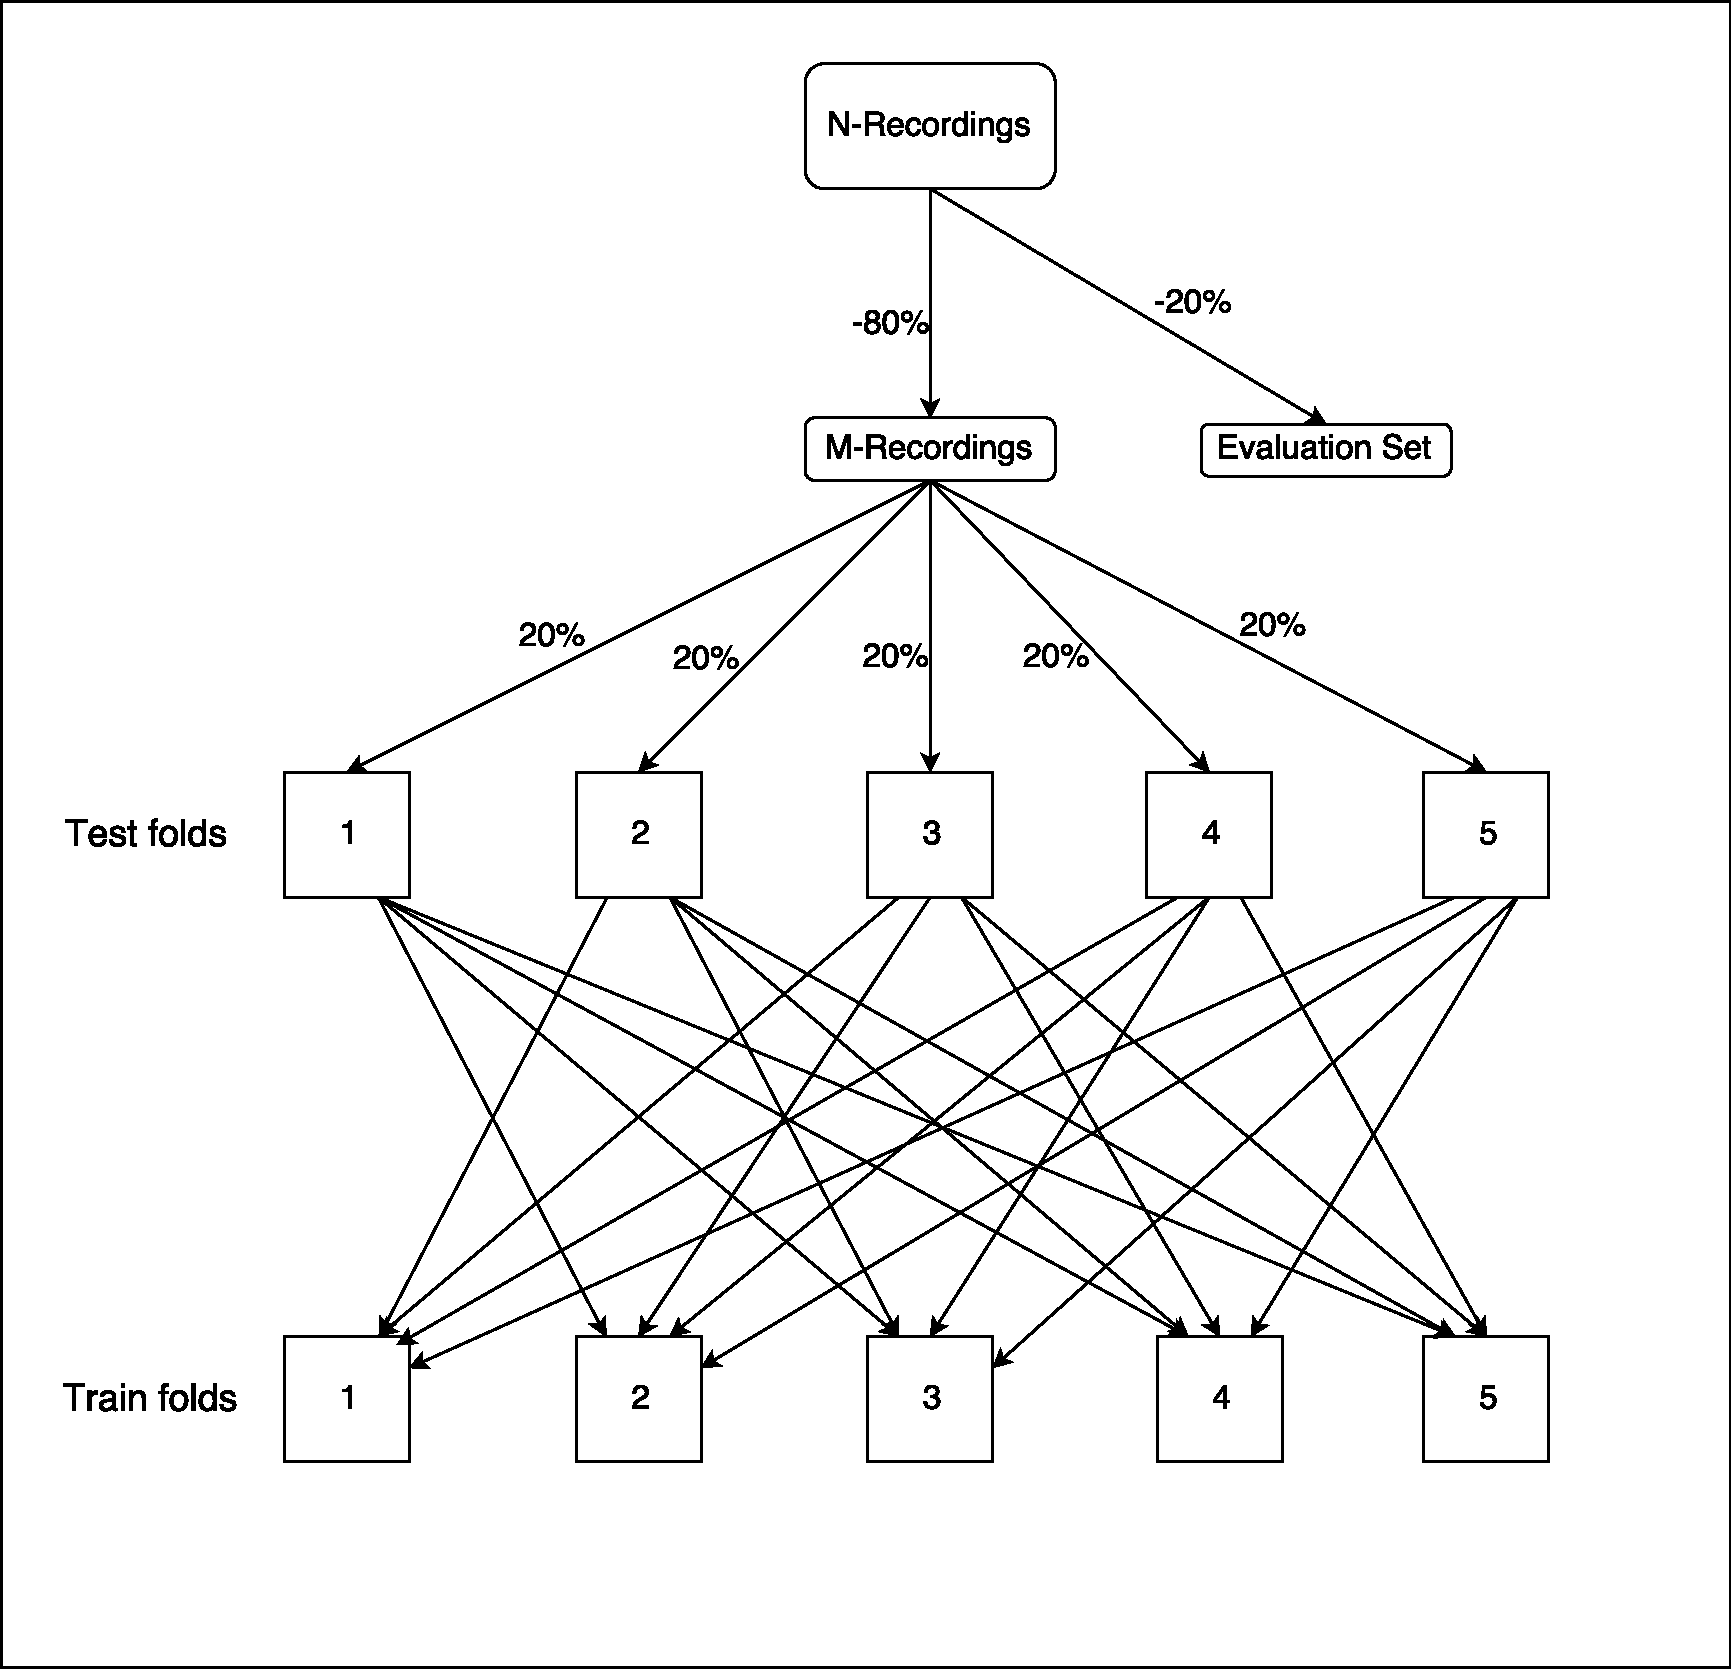
\includegraphics[width=15cm,left,keepaspectratio]{figures/data_division}
\caption{Division of recording into 5 folds}
\label{fig:division_into_5_folds}
\end{figure}

\section{Windowing}
Windowing is a common technique in machine learning to improve the detection accuracies. It is a procedure that is applied to the training and testing data before they are fed into the machine learning and thus it can be universally applied, independently of the  classification algorithm  in use  \cite{dietterich_machine_2002}. \\
In order to forward the data into the machine learning algorithm we often have to apply windowing to the data in order to properly format them as an input. In our experiments we acquire raw EMG data from the Myo that are captured at a fixed sampling frequency of 200 Hz. We force the classifier to take a certain perspective on the problem by defining a sample to consist of this set. 
Windowing is a way to avoid the problem of comparatively long ranges of samples by reducing the input vector's length. We define a window length \textit{w} and reshape the input vector in such a way that each input vector contains \textit{w} sensor readings. For example, if we acquire the EMG data of one Myo armband and assume a window of size \textit{w} = 10, each input vector contains not just 8, but 80 values, corresponding to 10 consecutive readings of the 8 EMG sensors in one Myo armband.\\
With this technique, each output value corresponds to larger set of sensor readings, more actual muscle activity is mapped to a gesture. This seems to be reasonable approach when looking at the vast differences in resolution: up to 200 sensor readings per second vs. one gesture change every few seconds. In such a manner, this approach forces the classifier to look at the data through a window that shows a more expressive excerpt of the input data.\\
The disadvantage that comes with windowing is that every value \textit{w} that is used creates an artificial connection between those \textit{w} values of input data that either may or may not be relevant to determine the corresponding output values. For example, if the window length \textit{w} is wide, a window can contain data that belongs to multiple gestures. On the contrary, if the window is narrow it may not contain the necessary number of samples to characterize succesfully the multiple gestures. That is why \textit{w} needs to be chosen carefully.\\
A solution to overcome this particular problem of windowing is to create \textit{overlapping} windows. Without overlapping windows each sample is somehow treated with the same weight. However, when someone observes the extracted features from two consecutive frames the change of property between the frames may induce a discontinuity. With the overlapping though, some $x_i$ of the original input vector will land in multiple windows. With this way, each measurement can be viewed twice but in a different context.\\
Depending on the value \textit{o} which is bounded with $0 \leq o \leq w-1$ this can increase  the size of the input vector. At the cost of larger vector sizes and effectively more computation time, overlapping windows  can reduce the impact of the artificial connection between values that is introduced by windowing. \\
\subsection{Windowing in current work}
In our case, Fig. \ref{fig:windowing} states that we take each train, test and evaluation sets and we apply a window of 128 length with a step of one to each recording. For the sake of computation time we changed the step from one to 64 for the later experiments. Each row of each recording consists of nine columns where the first column is the timestamp and the rest eight columns are the indicators from the eight \ac{EMG} sensors. All the produced 128-length windows are concatenated vertically in a final array.
\begin{figure}[h!]
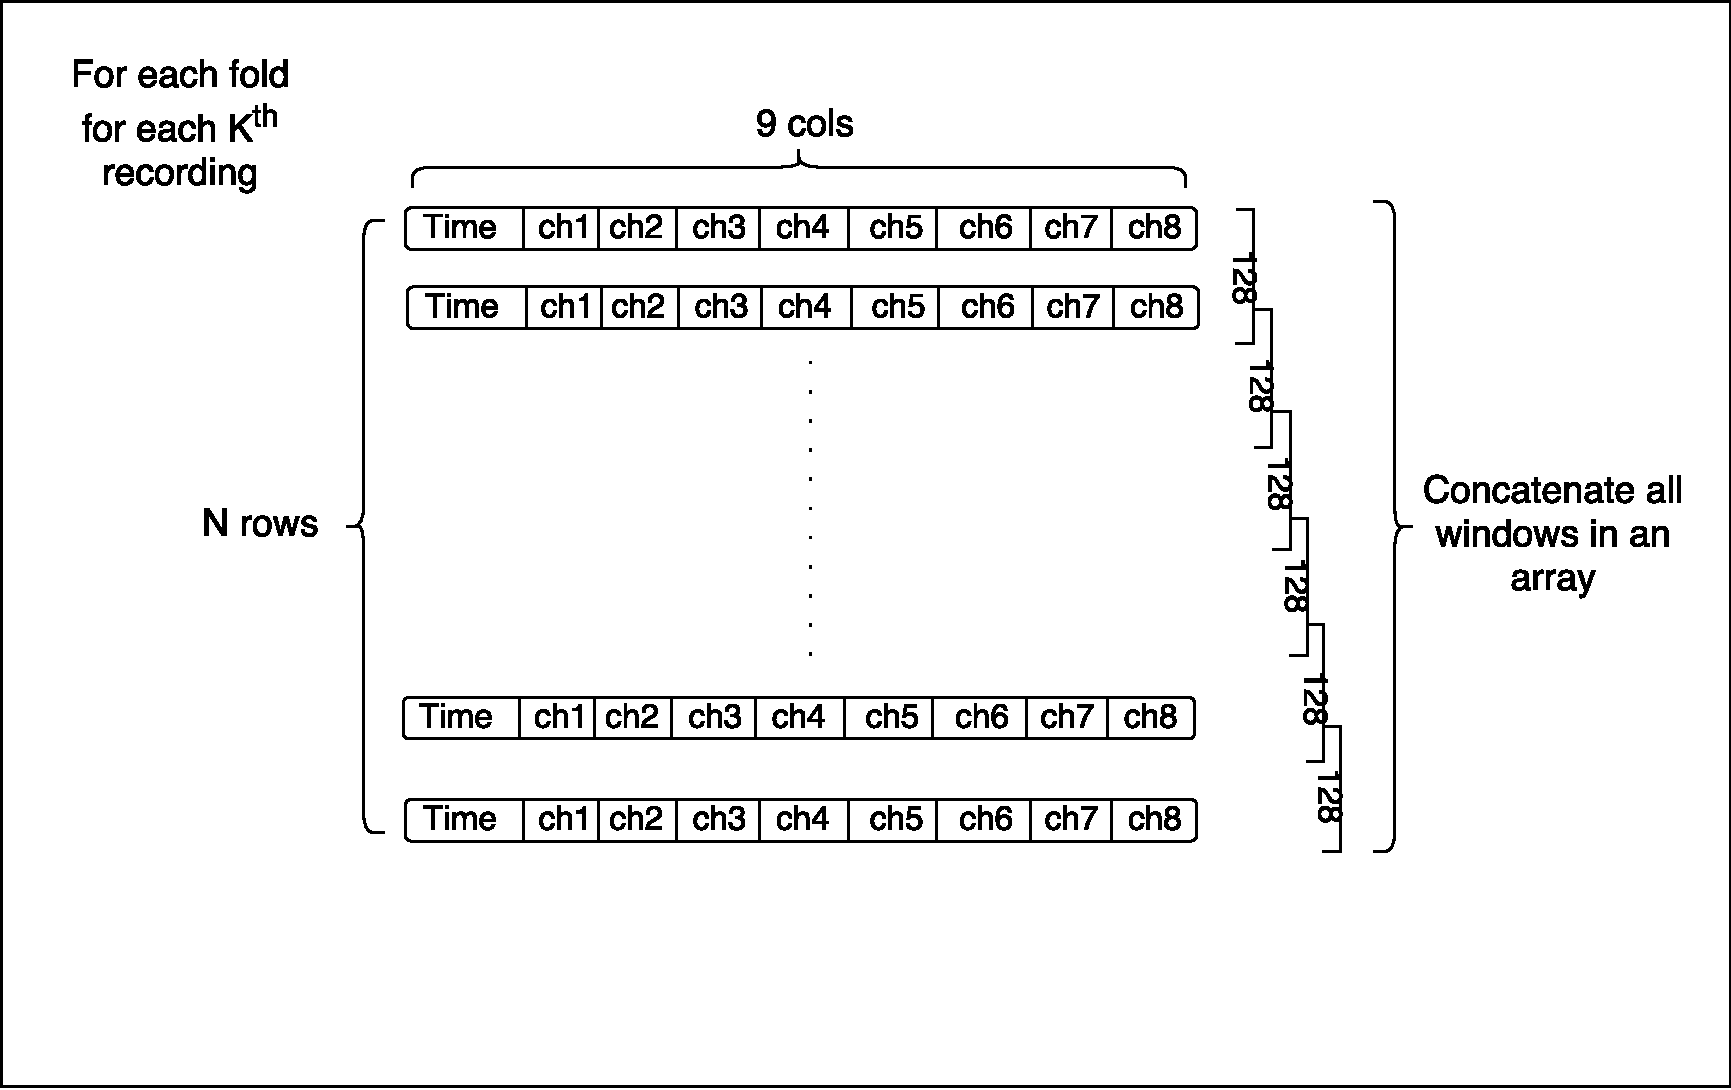
\includegraphics[width=15cm,left,keepaspectratio]{figures/windowing}
\caption{Windowing}
\label{fig:windowing}
\end{figure}

\section{Feature extraction}
The information extracted from the \ac{EMG} signals, which are represented in a feature vector, is chosen to help in minimizing the classification error which show us which of the selected features have the possibility for the most efficient identification of the each finger gesture. \\

In this section we are going to explain further the methods we used to extract the features from the acquired EMG signals. 
\subsection{Moving average}
The moving average function, calculates a series of averages from successive segments of a series of values. A moving average is used with time series data to smooth out short-term fluctuations as our data are already noisy. The simple moving average is taken from an equal number of data points on either side of a central value. This requires using an odd number of values in the sample window. In our case, moving average is taken in a window size of five. The definition of the arithmetic mean is given by the following equation \cite{whittaker_calculus_1924}:
\begin{equation}
s_i = \frac{1}{n} \sum_{j=1}^{i+n-1}\alpha_j
\end{equation}
\subsection{Root mean square}
Root mean square (abbreviated RMS and sometimes called the quadratic mean) is the square root of the arithmetic mean of the squares of a set of values. The equation is following:
\begin{equation}
x_{RMS} = \sqrt{\frac{x_1^2+x_2^2+ \hdots + x_n^2}{n}} =
          \sqrt{\frac{\sum_{i=1}^{n}x_i^2}{n}} = \sqrt{\langle x^2 \rangle}
\end{equation}
where $\langle x^2 \rangle$ is the arithmetic mean of the series $x_i^2$ \cite{kenney_mathematics_2013}. If $x$ is a row or a column vector, $x_{RMS}$ is a real-valued scalar. 
\subsection{Short-time Fourier transform}
STFT is a well known technique in signal processing to analyze non-stationary signals. Particularly, STFT helps to analyze a small section of the signal over time thanks to the \textit{windowing} function applied (e.g., Hann, Gaussian) on the signal. Fig. \ref{fig:fft} shows us in brief how STFT works.
\begin{figure}[!htb]
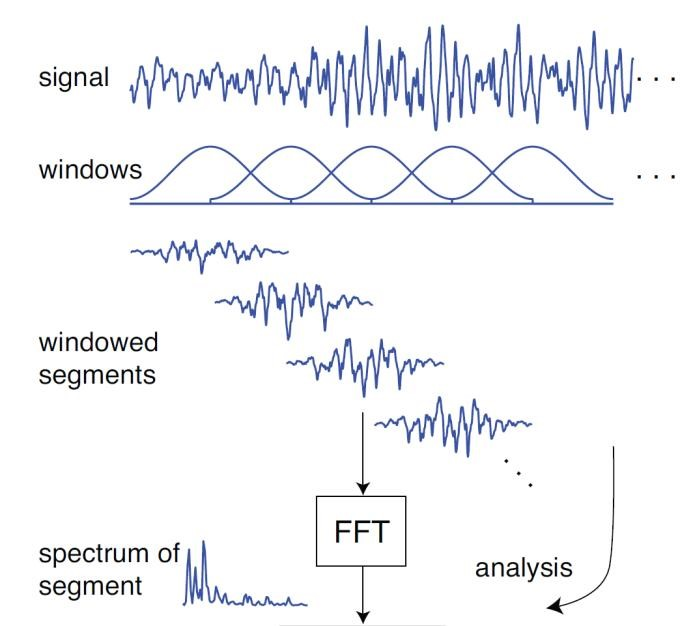
\includegraphics[width=10cm,center,keepaspectratio]{figures/fft}
\caption{Application of the STFT in the segmented windows \cite{sethares_rhythm_2007}}
\label{fig:fft}
\end{figure}
STFT maps a signal into a two-dimensional function of time and frequency. Each section, that means $x[n]w[n-m]$ is Fourier transformed, and the complex result is added to a matrix, which records magnitude and phase for each point in time and frequency. This can be expressed as:
\begin{equation}
\textbf{STFT}{x[n]}(m, \omega) \equiv X(m, \omega) = \sum_{n = - \infty}^{\infty}x[n]w[n-m]\exp^{-j\omega n}
\end{equation}
with signal $x[n]$ and window $w[n]$. STFT provides information about when and which frequencies in a signal occurs. One can obtain that information with a limited precision depending on the size of the window.  As the size of the time window is the same for all frequencies this constitutes a disadvantage and leads to cutting valuable information. To determine accurately time or frequency one need to vary the window size. The weak point of STFT is that whoever wants to use it will face the problem of resolution. Which means that there is a question of what window size should someone choose. Narrow windows offer good time resolution but poor frequency resolution. Wide windows offer good frequency resolution but poor time resolution \cite{polikar_wavelet_1996}. To visualize what we explained with words, in Fig. \ref{fig:spectrograms} we produce four spectrograms to emphasize between the different effect the window size of STFT has on the signal that is consisted from simple stationary sinusoidal waveforms joined together. The signal is sampled at frequency 400 Hz:
\begin{equation}
x(t) = \begin{cases}
      cos(2 \pi 10 t) & 0s \leq t < 5s \\
      cos(2 \pi 25 t) & 5s \leq t < 10s\\
      cos(2 \pi 50 t) & 10s \leq t < 15s \\
      cos(2 \pi 100 t) & 15s \leq t < 20s
\end{cases}
\end{equation}
\begin{figure}[!htb]
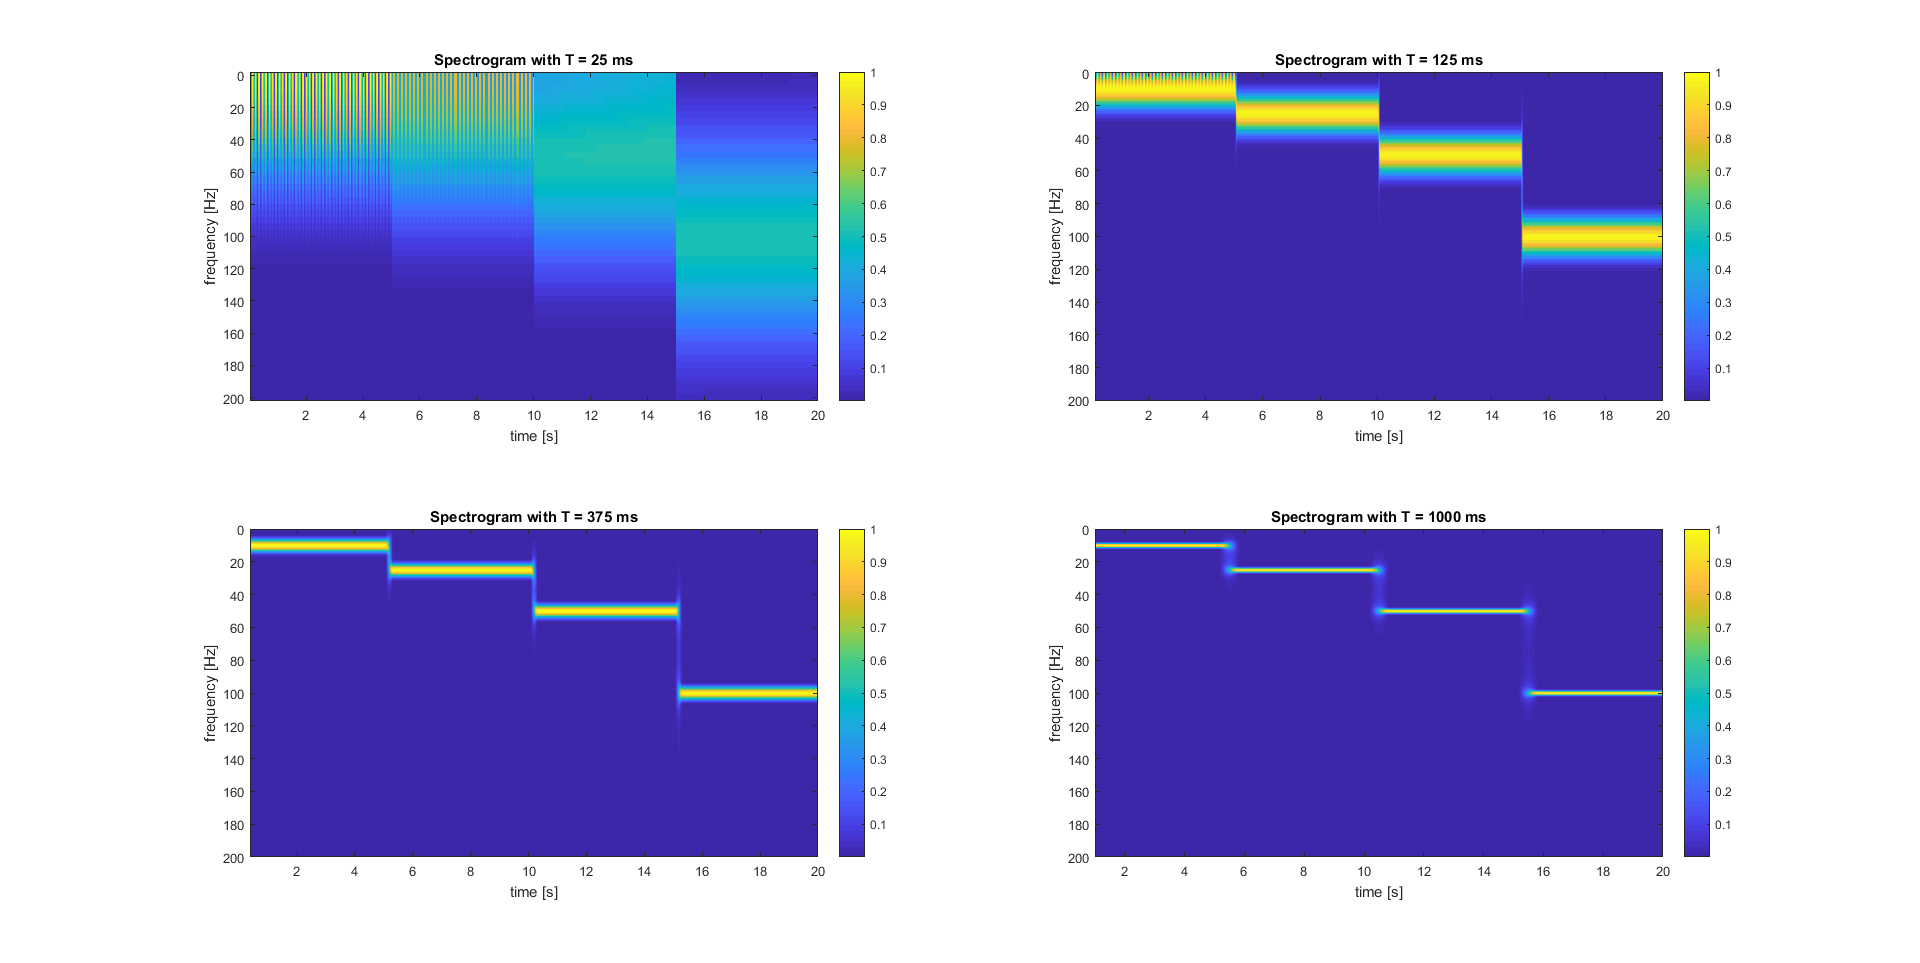
\includegraphics[width=20cm,center,keepaspectratio]{figures/spectrograms}
\caption{Spectrograms of the thumb extension}
\label{fig:spectrograms}
\end{figure}
As we can observe, with the 25 ms window we are able to say with great precision when the frequency of the signal changes but to identify which frequencies exist in the signal still remains a difficult task. On the contraty, with bigger window sizes such as with T = 1000 ms we can detect with great precision which frequencies exist in the signal while the determination of the periods when these frequencies happen is difficult to distinguish because of the blur.
\newpage
The spectrogram we used to visualize the STFT of the signals is generated by the squared magnitude of the STFT. The equation is following:
\begin{equation}
\textbf{spectrogram}\{x(t)\}(\tau, \omega) \equiv \left|X(\tau, \omega)\right|^2
\end{equation}
In the Fig. \ref{fig:STFT_ch7_ext} we can see the spectrogram of a signal coming from the thumb extension and in the Fig. \ref{fig:STFT_ch7_flx} we can see the spectrogram of a signal coming from the thumb flexion.
\begin{figure}[!htb]
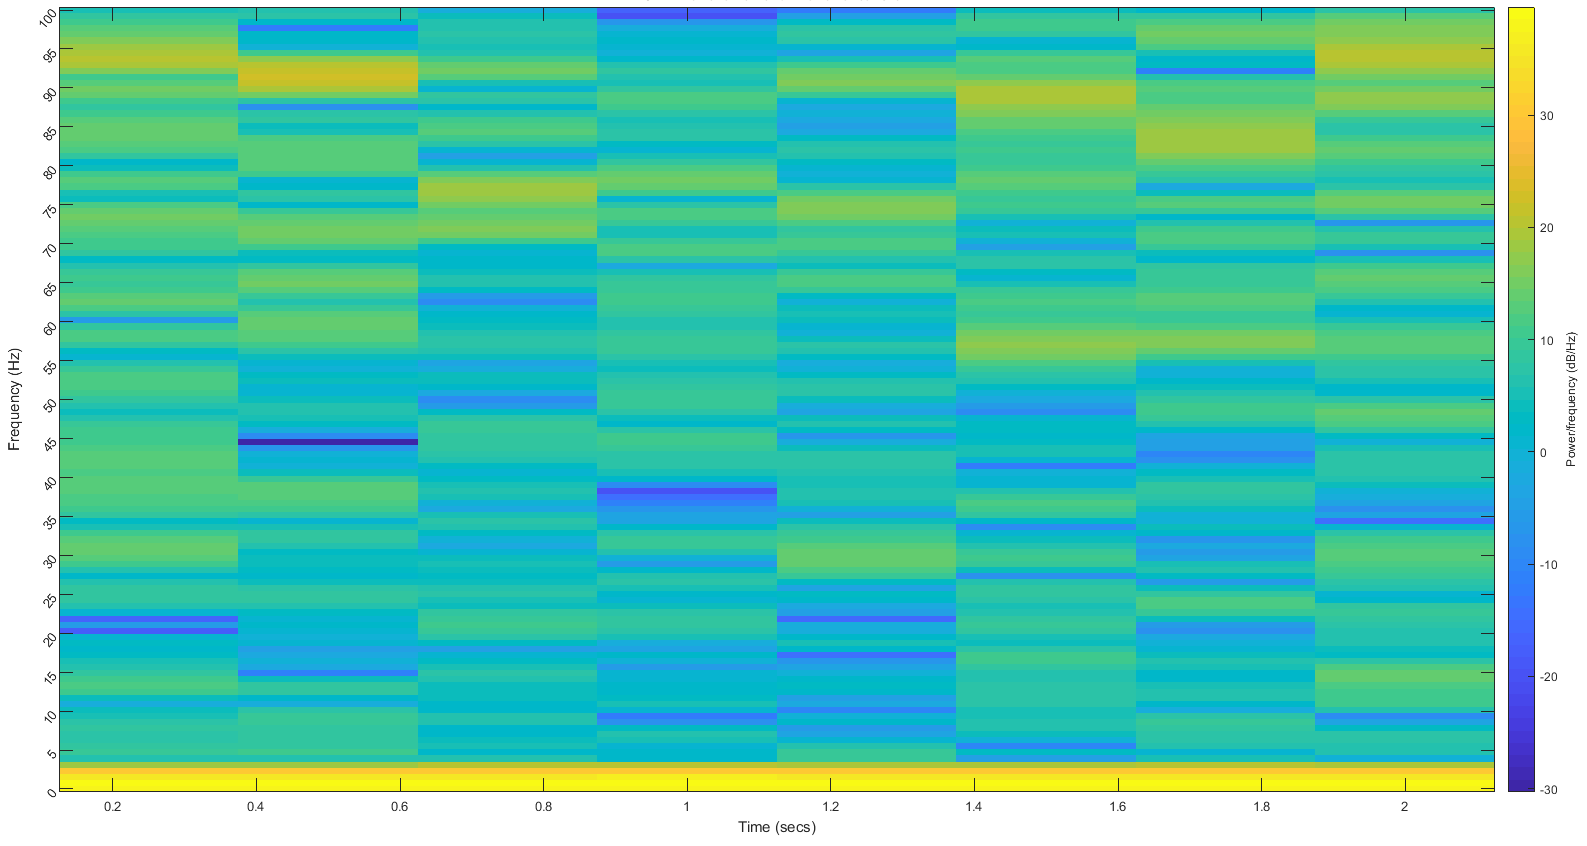
\includegraphics[width=16cm,left,keepaspectratio]{figures/STFT_ch7_ext}
\caption{Spectrogram of the thumb extension from Myo's 7th channel}
\label{fig:STFT_ch7_ext}
\end{figure}
\begin{figure}[!htb]
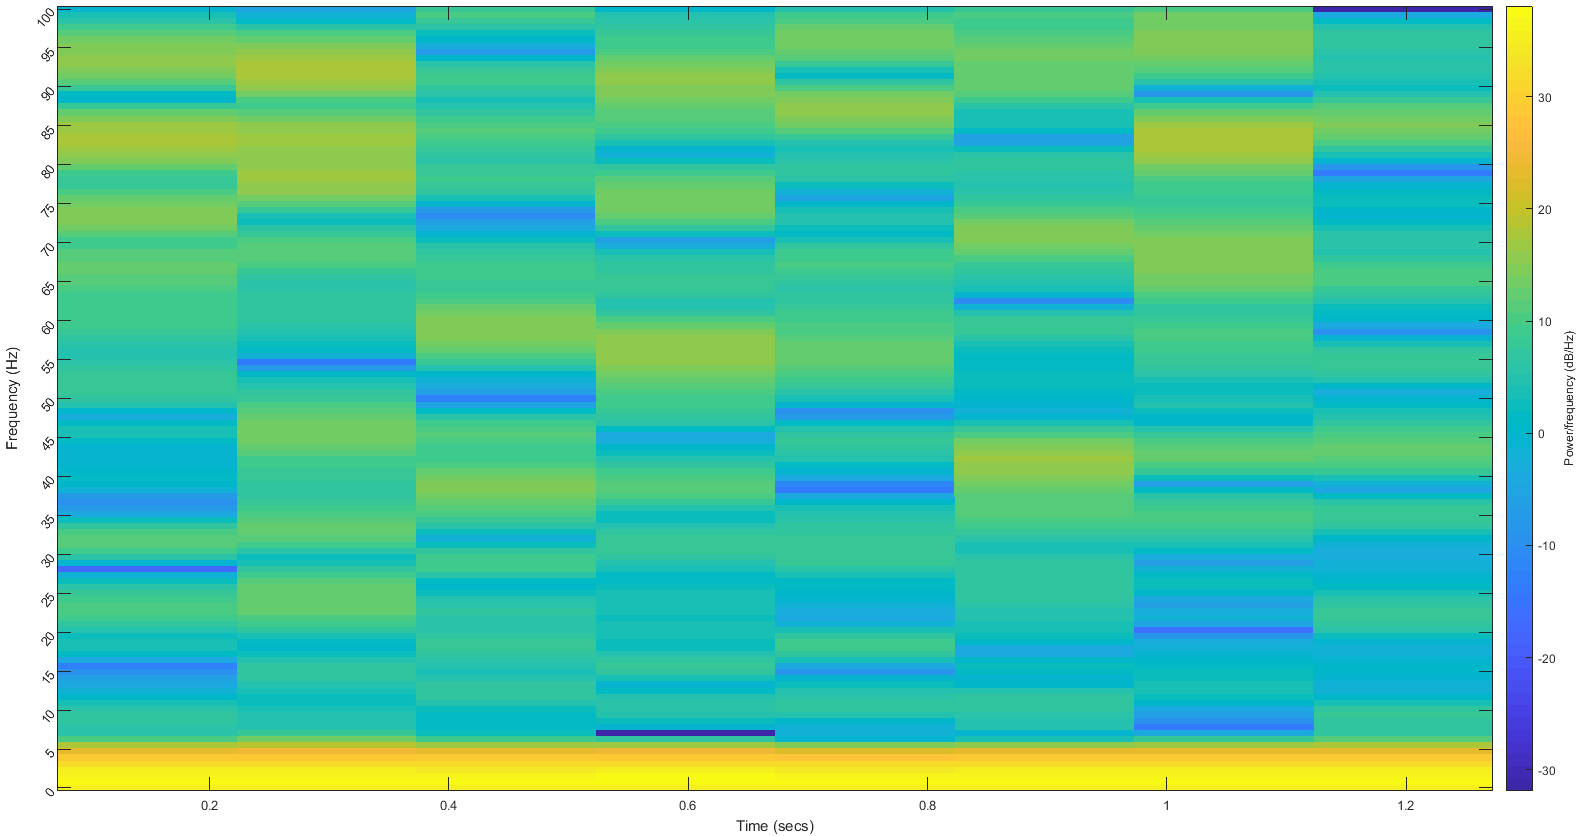
\includegraphics[width=16cm,left,keepaspectratio]{figures/STFT_ch7_flx}
\caption{Spectrogram of the thumb flexion from Myo's 7th channel}
\label{fig:STFT_ch7_flx}
\end{figure}
The spectrogram can be represented as a visual heat map where the horizontal axis represents the time axis and the vertical axis represents the frequency axis. In the above image the darker colors visualize for a particular time point and a particular frequency low magnitude. So, the darker the colors the lower the magnitude and similarly the higher in magnitude the frequency component is, the lighter the color.
\subsection{Wavelet Analysis}
Wavelet analysis (also called wavelet theory or just wavelets) has attracted much attention in signal processing. In order to overcome the resolution problem with the fixed window size in Fourier Transform a different approach is employed. Like Fourier analysis, wavelet analysis deals with expansion of functions in terms of a set of basis functions. Unlike Fourier analysis, wavelet analysis expands functions not in terms of trigonometric polynomials but in terms of wavelets, which are generated in the form of translations and dilations of a fixed function called the mother wavelet \cite{lee_wavelet_1994}. \\
A wavelet is a little wave oscillation with an amplitude that begins at zero increases and decreases back to zero. The original signal is convoluted with the wavelets. With this way, useful information is extracted from the raw signals. \\
\begin{figure}[H]
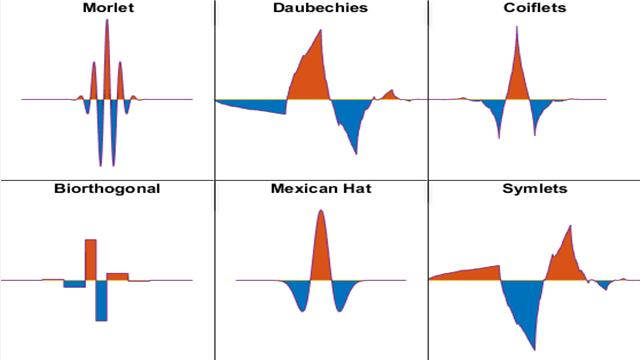
\includegraphics[width=13cm,center,keepaspectratio]{figures/wavelets}
\caption{Wavelet families \cite{fig:wavelets}}
\label{fig:wavelets}
\end{figure}
\subsection{Continuous wavelet transform}
The formula for the continuous wavelet transform is:
\begin{equation}
\textbf{CWT}^\psi_\chi(\tau,s) = \Psi^{\psi}_{\chi}(\tau,s) = \frac{1}{\sqrt{\left|s\right|}}\int x(t) \psi ^{\ast} (\frac{t - \tau}{s})dt
\label{Eq:CWT}
\end{equation}
where $\tau $ is translation (location of the window) and $s$ is scale. $\psi ^{\ast} (\frac{t - \tau}{s})$ is the \textbf{mother wavelet} which we will explain further later. \\
The most significant difference between STFT and wavelets is that the width of the window is changed in wavelet analysis whereas the window used by STFT is fixed \cite{giurgiutiu_comparison_2003}. For local areas with high frequencies the window size will be shorter whereas for local areas with low frequencies the window size will be longer. 
The term \textbf{mother wavelet} gets its name by two important properties. Firstly, wavelet as it is a small wave (finite length), and mother because all functions with different regions of support stem from a main function, the mother wavelet. This means that mother wavelet acts as a prototype for generating other functions. The translation term is related to the location of  the window while it is shifting through the signal. Thus, translation term corresponds to the time information. As we can observe there is no frequency component in the Eq. \ref{Eq:CWT}. Instead, we have the scale parameter which is $\frac{1}{frequency}$. In terms of frequencies, low frequencies (high scales) correspond to a macroscopic information of the entire signal, whereas high frequencies (low scales) correspond to a microscopic detailed information of the signal. High scales (low frequencies) last for the entire duration of the signal while low scales (high frequencies) do not last for the entire duration of the signals but appear from time to time like short bursts.  \\
\subsection{Discrete wavelet transform}
The discrete wavelet transform (\ac{DWT}) is an implementation of the wavelet transform using a discrete set of the wavelet scales and translations obeying some rules. DWT is simply a sampled version of \ac{CWT}. The Discrete Wavelet Transform (\ac{DWT}) provides sufficient information for synthesis and analysis of the original signal. \ac{DWT} is similar to the Fourier transform in that it is a decomposition of a signals in terms of a basis set of functions. In Fourier Transform, the basis set consists of sines and cosines and the expansions has one parameter which is the window length. In wavelet transform, the expansion has two parameters and the wavelets are generated from a single mother wavelet using dilation and offsets corresponding to the two parameters. The formula for the discrete wavelet transform is given by:
\begin{equation*}
f(t) = \sum_s\sum_{\tau} c_{s\tau} \psi_{s\tau} (t)
\end{equation*}
where the two-parameter expansion coefficients are given by
\begin{equation*}
c_{s \tau} = \int f(t) \psi_{s \tau}(t)dt
\end{equation*}
and the wavelets obey the situation
\begin{equation*}
\psi_{s\tau}(t) = 2^{\frac{s}{2}} \Psi(2^s t-\tau)
\end{equation*}
Here $\Psi$ is the mother wavelet, $s$ is the scale parameter and $\tau$ is the translate parameter. DWT applies the same idea as CWT. CWT is a correlation between a wavelet at different scales and the signal with the scale (or frequency) being used as a measure of similarity. By scaling the analysis window, shifting it in time, multiplying it and integrating it over all times, we acquire the CWT of a signal. \\
In the discrete case, filters of different cutoff frequencies are used to analyze the signal at different scales. The signal is passed through a series of high pass filters to analyze the high frequencies and it is passed through a series of low pass filters to analyze the low frequencies. The resolution of the signal, which is the amount of detail in the signal, is changed by the different filter operations and the scale is changed by the upsampling and the downsampling (subsampling). Subsampling a signal means that we reduce the sampling rate or removing some samples from the signal whereas upsampling means that we increase the sampling rate by adding new samples to the signal.
\begin{figure}[!htb]
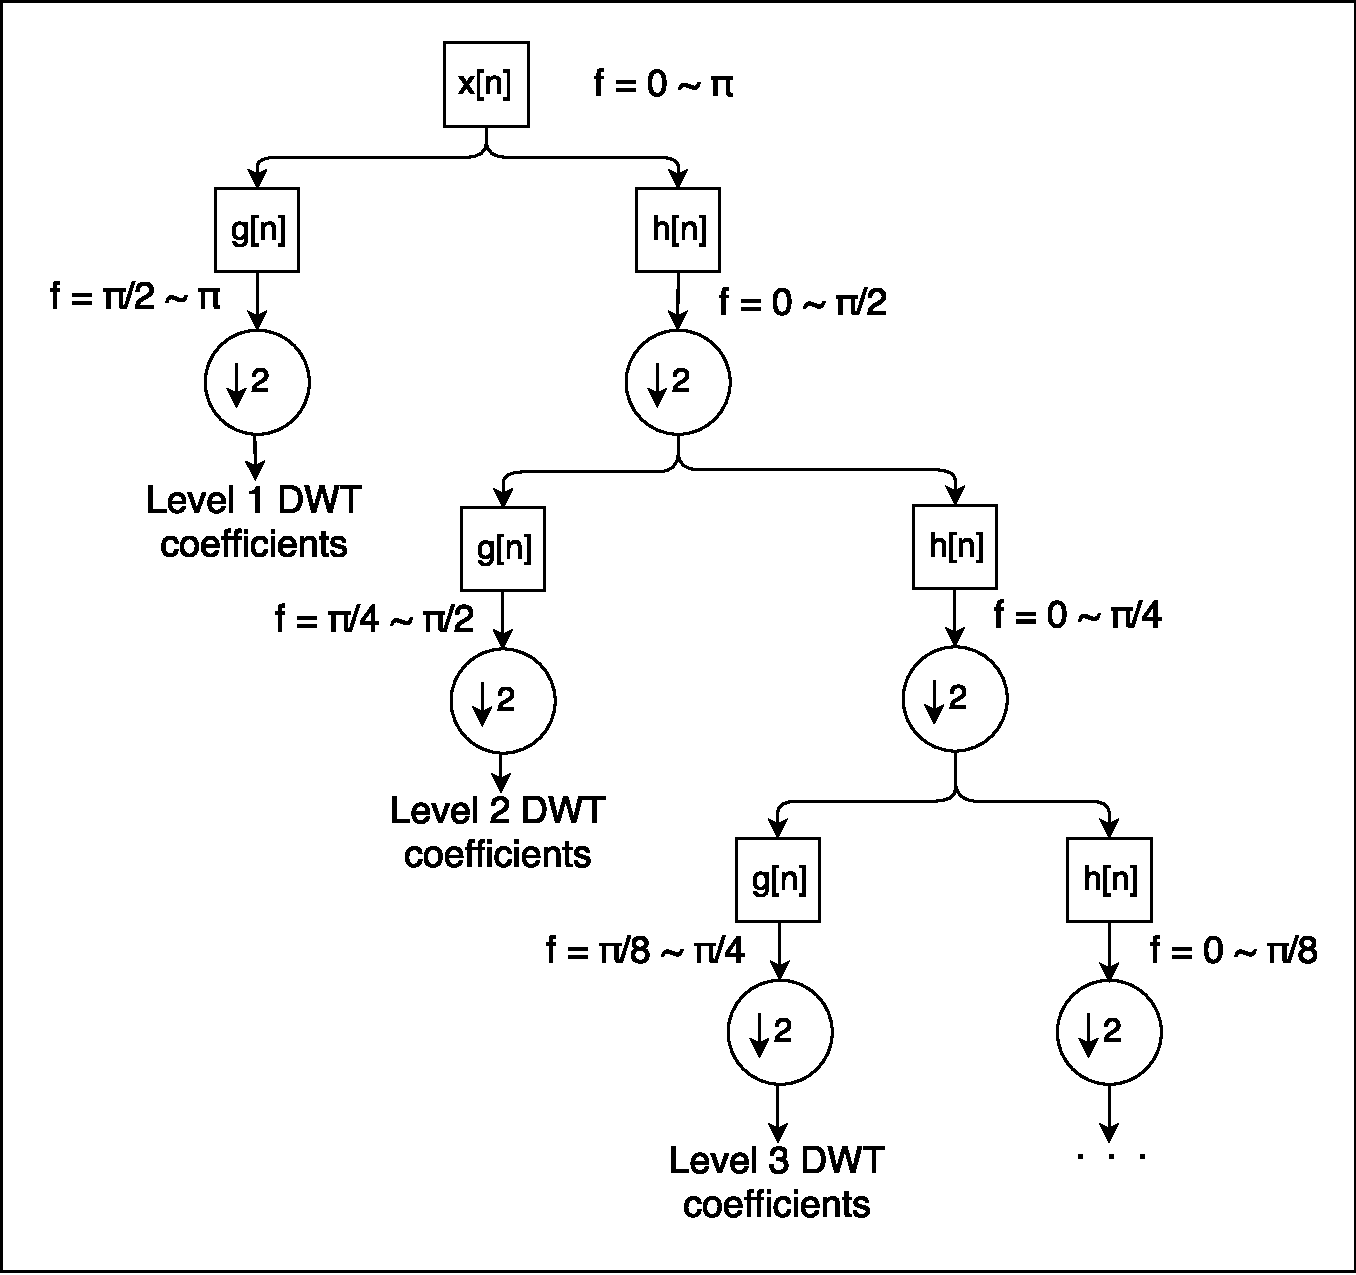
\includegraphics[width=15cm,left,keepaspectratio]{figures/subbandcoding}
\caption{The subband coding algorithm}
\label{fig:subbandcoding}
\end{figure}
The procedure starts with passing this signal through a half band digital lowpass filter with impulse response $h[n]$. The mathematical operation of convolution corresponds to filtering the signal with the impulse response of the filter. The convolution in discrete time is defined as:
\begin{equation*}
x[n] \circledast h[n] = \sum_{k=-\infty}^\infty x[k] \cdot h[n-k]
\end{equation*}
The half band lowpass filter removes all frequencies that are above half of the highest frequency in the signal. After passing the half band lowpass filter, half of the samples are eliminated thus leading to a subsampling of the signal by two, causing it to remain with half the number of points. Resolution is related to the amount of the information in the signal and therefore resolution is halved after the filtering operations. This causes the scale to double. This procedure can be expressed as:
\begin{equation*}
y[n] = \sum_{k=-\infty}^\infty h[k] \cdot x[2n-k]
\end{equation*}
According to the \ref{fig:subbandcoding} DWT employs two sets of functions, the scaling and the wavelet functions which correspond to low and highpass filters. These filters with the different frequency bands and with different resolutions, decompose the signal into a coarse approximation and detail information \cite{polikar_wavelet_1996}. The decomposition is obtained by applying successively highpass and lowpass filtering on the time domain signal.\\
The raw signal $x[n]$ is passed through a halfband highpass filter $g[n]$ and a lowpass filter $h[n]$. According to the Nyquist's rule, after the filtering, half of the samples are eliminated, since the signal has now a highest frequency of $p/2$ radians instead of $p$. This composes one level of decomposition and can be expressed as:
\begin{equation*}
y_{high}[k] = \sum_n x[n]g[2k - n]
y_{low}[k] = \sum_n x[n]h[2k - n]
\end{equation*}
where $y_{high}[k]$ and $y_{low}[k]$ are the outcomes of the highpass and lowpass filter after subsampling by 2.\\
Since only half of the number of the samples characterizes the raw signal, the decomposition halves the time resolution whereas the frequency resolution is doubled since the frequency band of the signal spans half the previous frequency band. At every level, the filtering and the subsampling half the number of samples (hence half the time resolution) and half the frequency band spanned (hence double the frequency resolution) \cite{polikar_wavelet_1996}. In the Fig. \ref{fig:subbandcoding} $h[n]$ $g[n]$ are lowpass and highpass filters and the bandwidth of the signal at every level is denoted with ``f''.\\
The most prominent frequencies in the raw signal will have the biggest amplitude in the DWT. The difference between DWT and the Fourier transform is that the time localization will be preserved. The time localization will have a different resolution depending on the current level we use for the DWT. The length of the signal determines the number of levels that the signal can be decomposed to. For example, if the signal length is 1024, ten levels of decomposition are possible \cite{polikar_wavelet_1996}. \\
If the main information is located in the high frequencies, the time localization will be more precise since higher frequencies are characterized by more number of samples. If the main information is located in the low frequencies, the time localization is less precise, since a small number of samples express the raw signal at low frequencies.\\
\subsubsection{Haar wavelet: An example of wavelet function}
The haar wavelet is the simplest kind of wavelet function. The haar wavelet is conceptually simple, memory efficient and computationally cheap. The haar transform also, does not have overlapping windows. Its formula is the following:
\[
\phi (t)
\begin{cases}
         1, & \text{if  } 0 \leq t \leq 1 \\
         0, & \text{otherwise}
\end{cases}         
\]
If we define the function $\psi(t)$ as $\psi(t) = \phi(2t) - \phi(2t-1)$, we can obtain the following function:
\[
\psi(t) = 
\begin{cases}
1, & \text{if } 0 < t \leq \frac{1}{2} \\
-1, & \text{if } \frac{1}{2} < t \leq 1 \\
0, & \text{otherwise }
\end{cases}
\]
The function $\phi(t)$ is the Haar scaling function, and $\psi(t)$ is the Haar wavelet. \cite{lee_wavelet_1994}
\subsection{Feature extraction in current work}
In Fig. \ref{fig:feature_extraction} we show that before proceeding with the preprocessing of the former matrix we created, we discard the time vector as we are not going to use the timestamps. Subsequently, we extract each 128-row-size segment from the matrix and we filter it with each feature we selected. After the feature extraction of each segment we convert the resulting matrix into a row. Each row represents the matrix from a preprocessed 128-row-size segment. The produced number of columns is variable for each different feature. We repeat all the aforementioned processes, for the data which are included in each of the folds. 
\begin{figure}[h!]
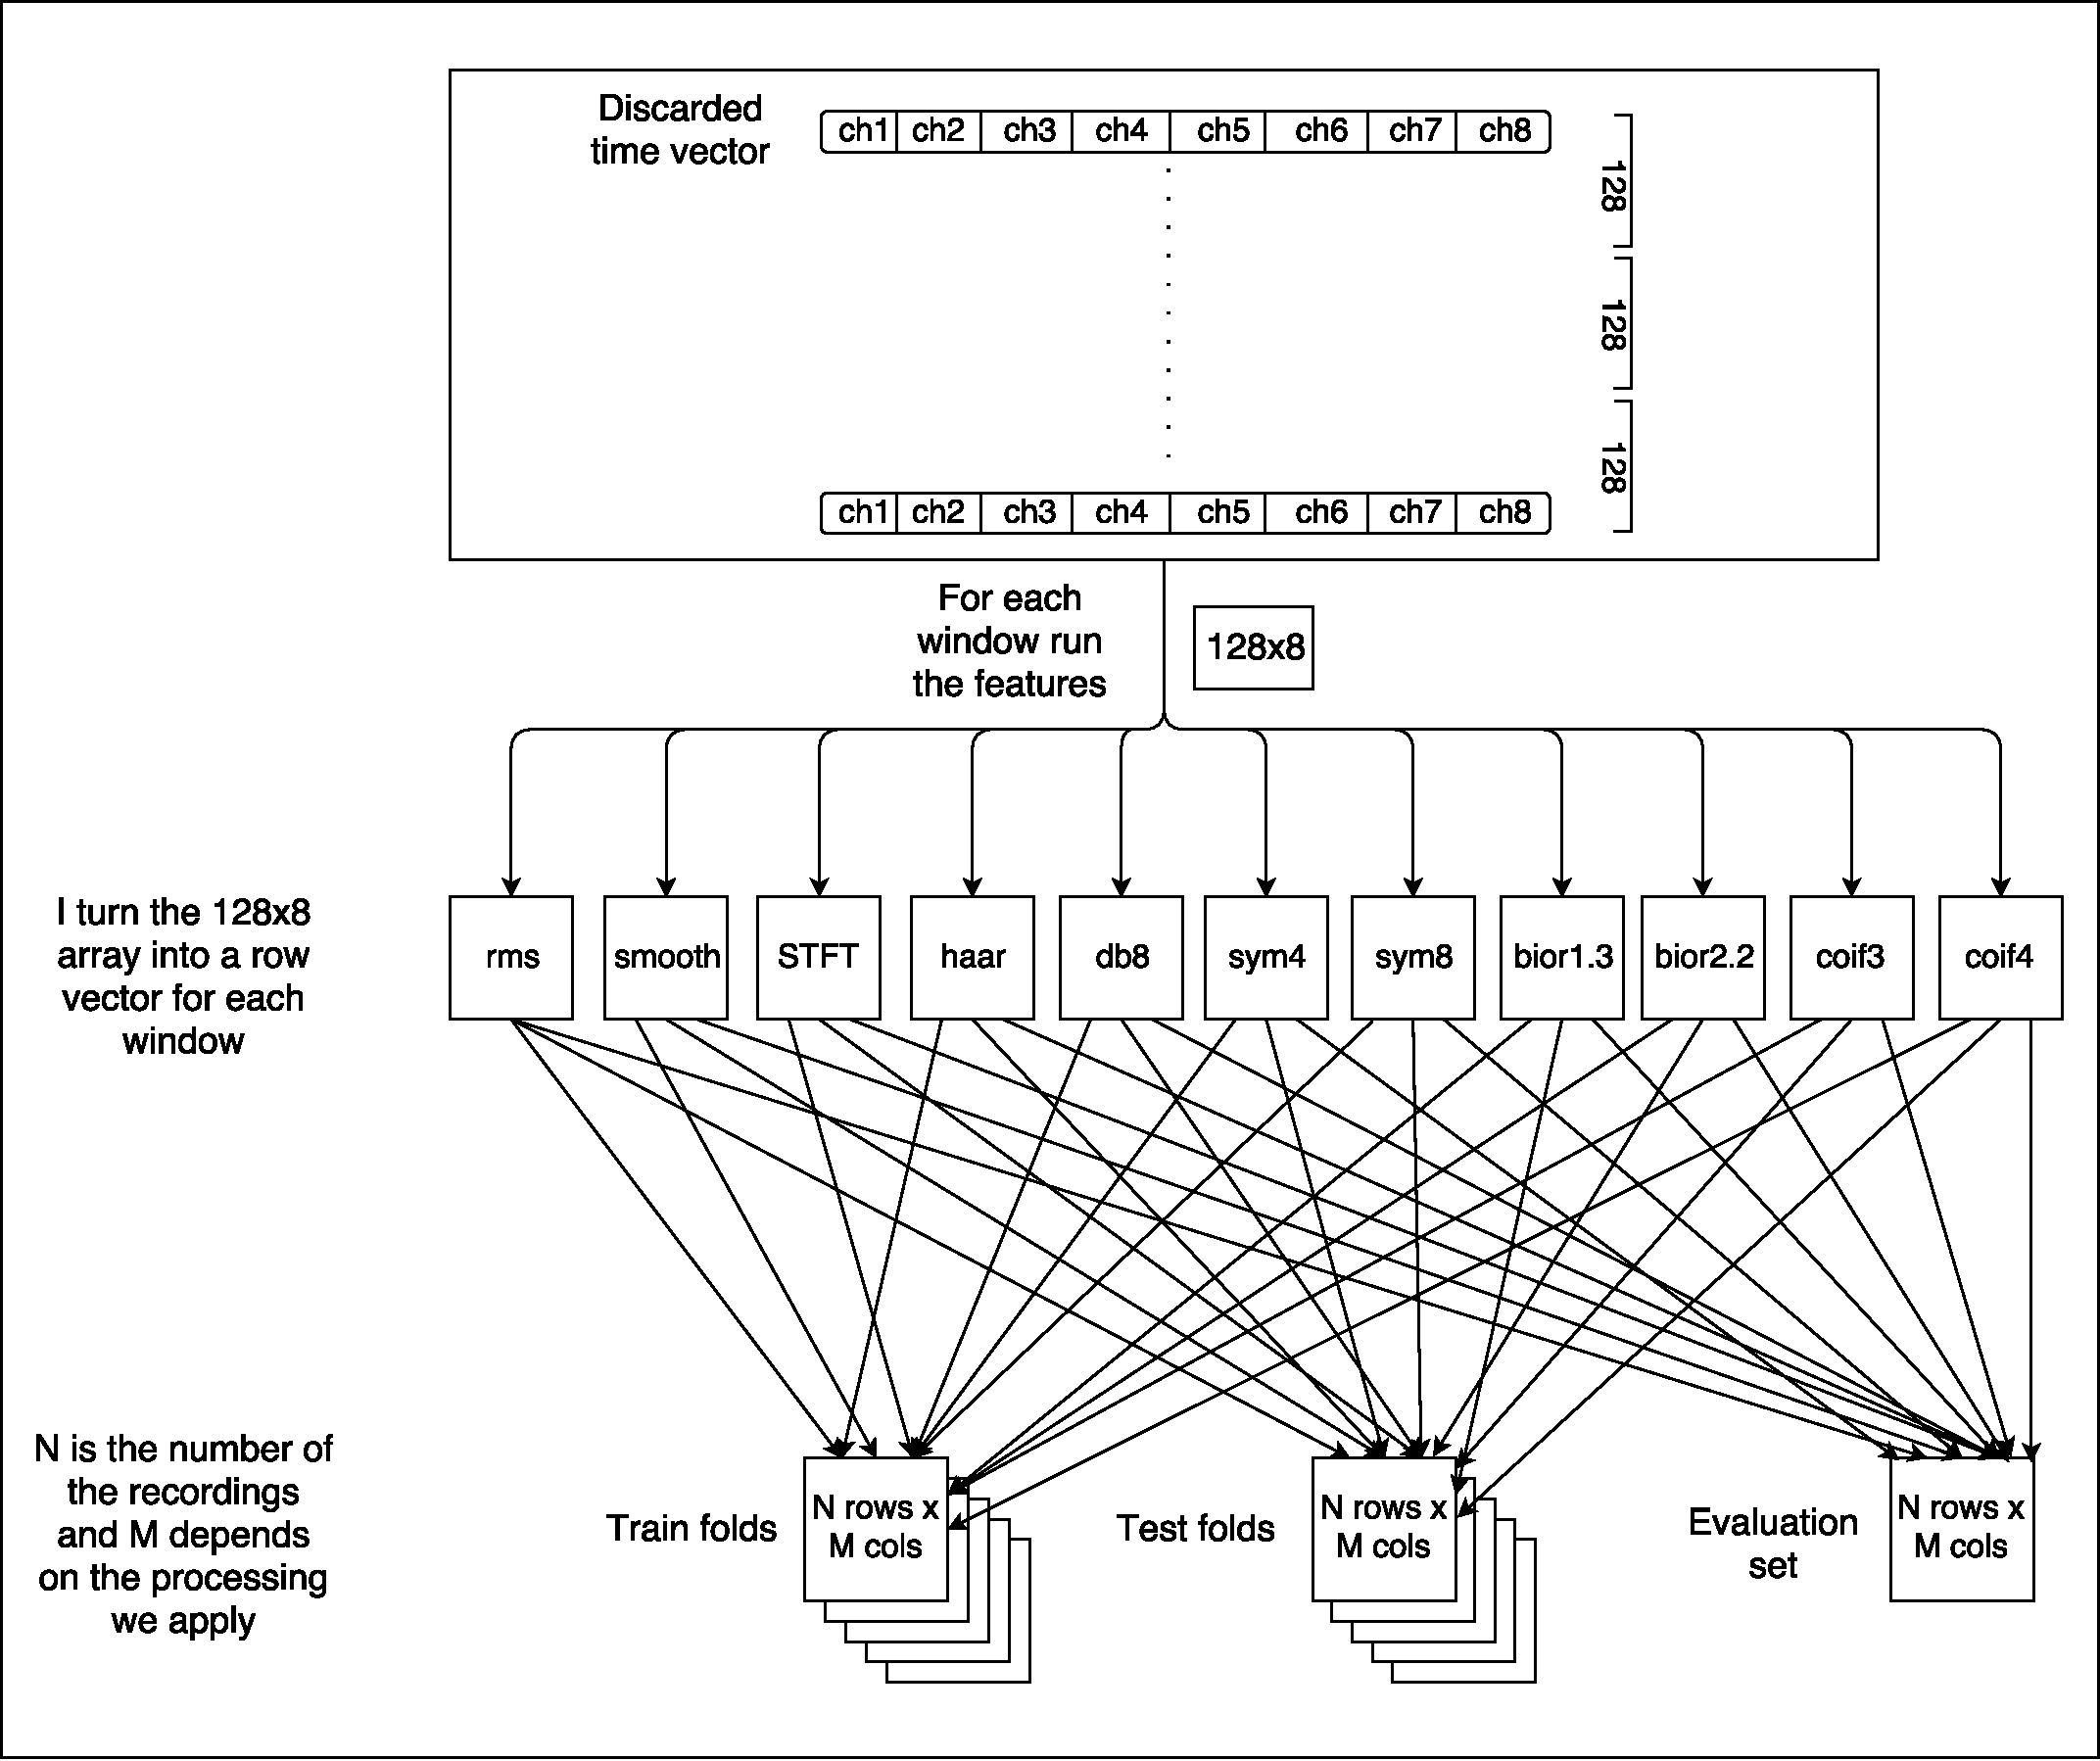
\includegraphics[width=15cm,left,keepaspectratio]{figures/feature_extraction}
\caption{Feature extraction}
\label{fig:feature_extraction}
\end{figure}
\section{Training and classification}
In Fig.\ref{fig:train_classification} we see that for each movement for feature from the train folds we train the SVM, \ac{ANN} classifiers. After the training has happened we use the test folds we previously created and we classify them with the newly trained network. After, that classification we calculate the accuracy which is calculated by the extraction of mean-squared-error from one.
\begin{figure}[h!]
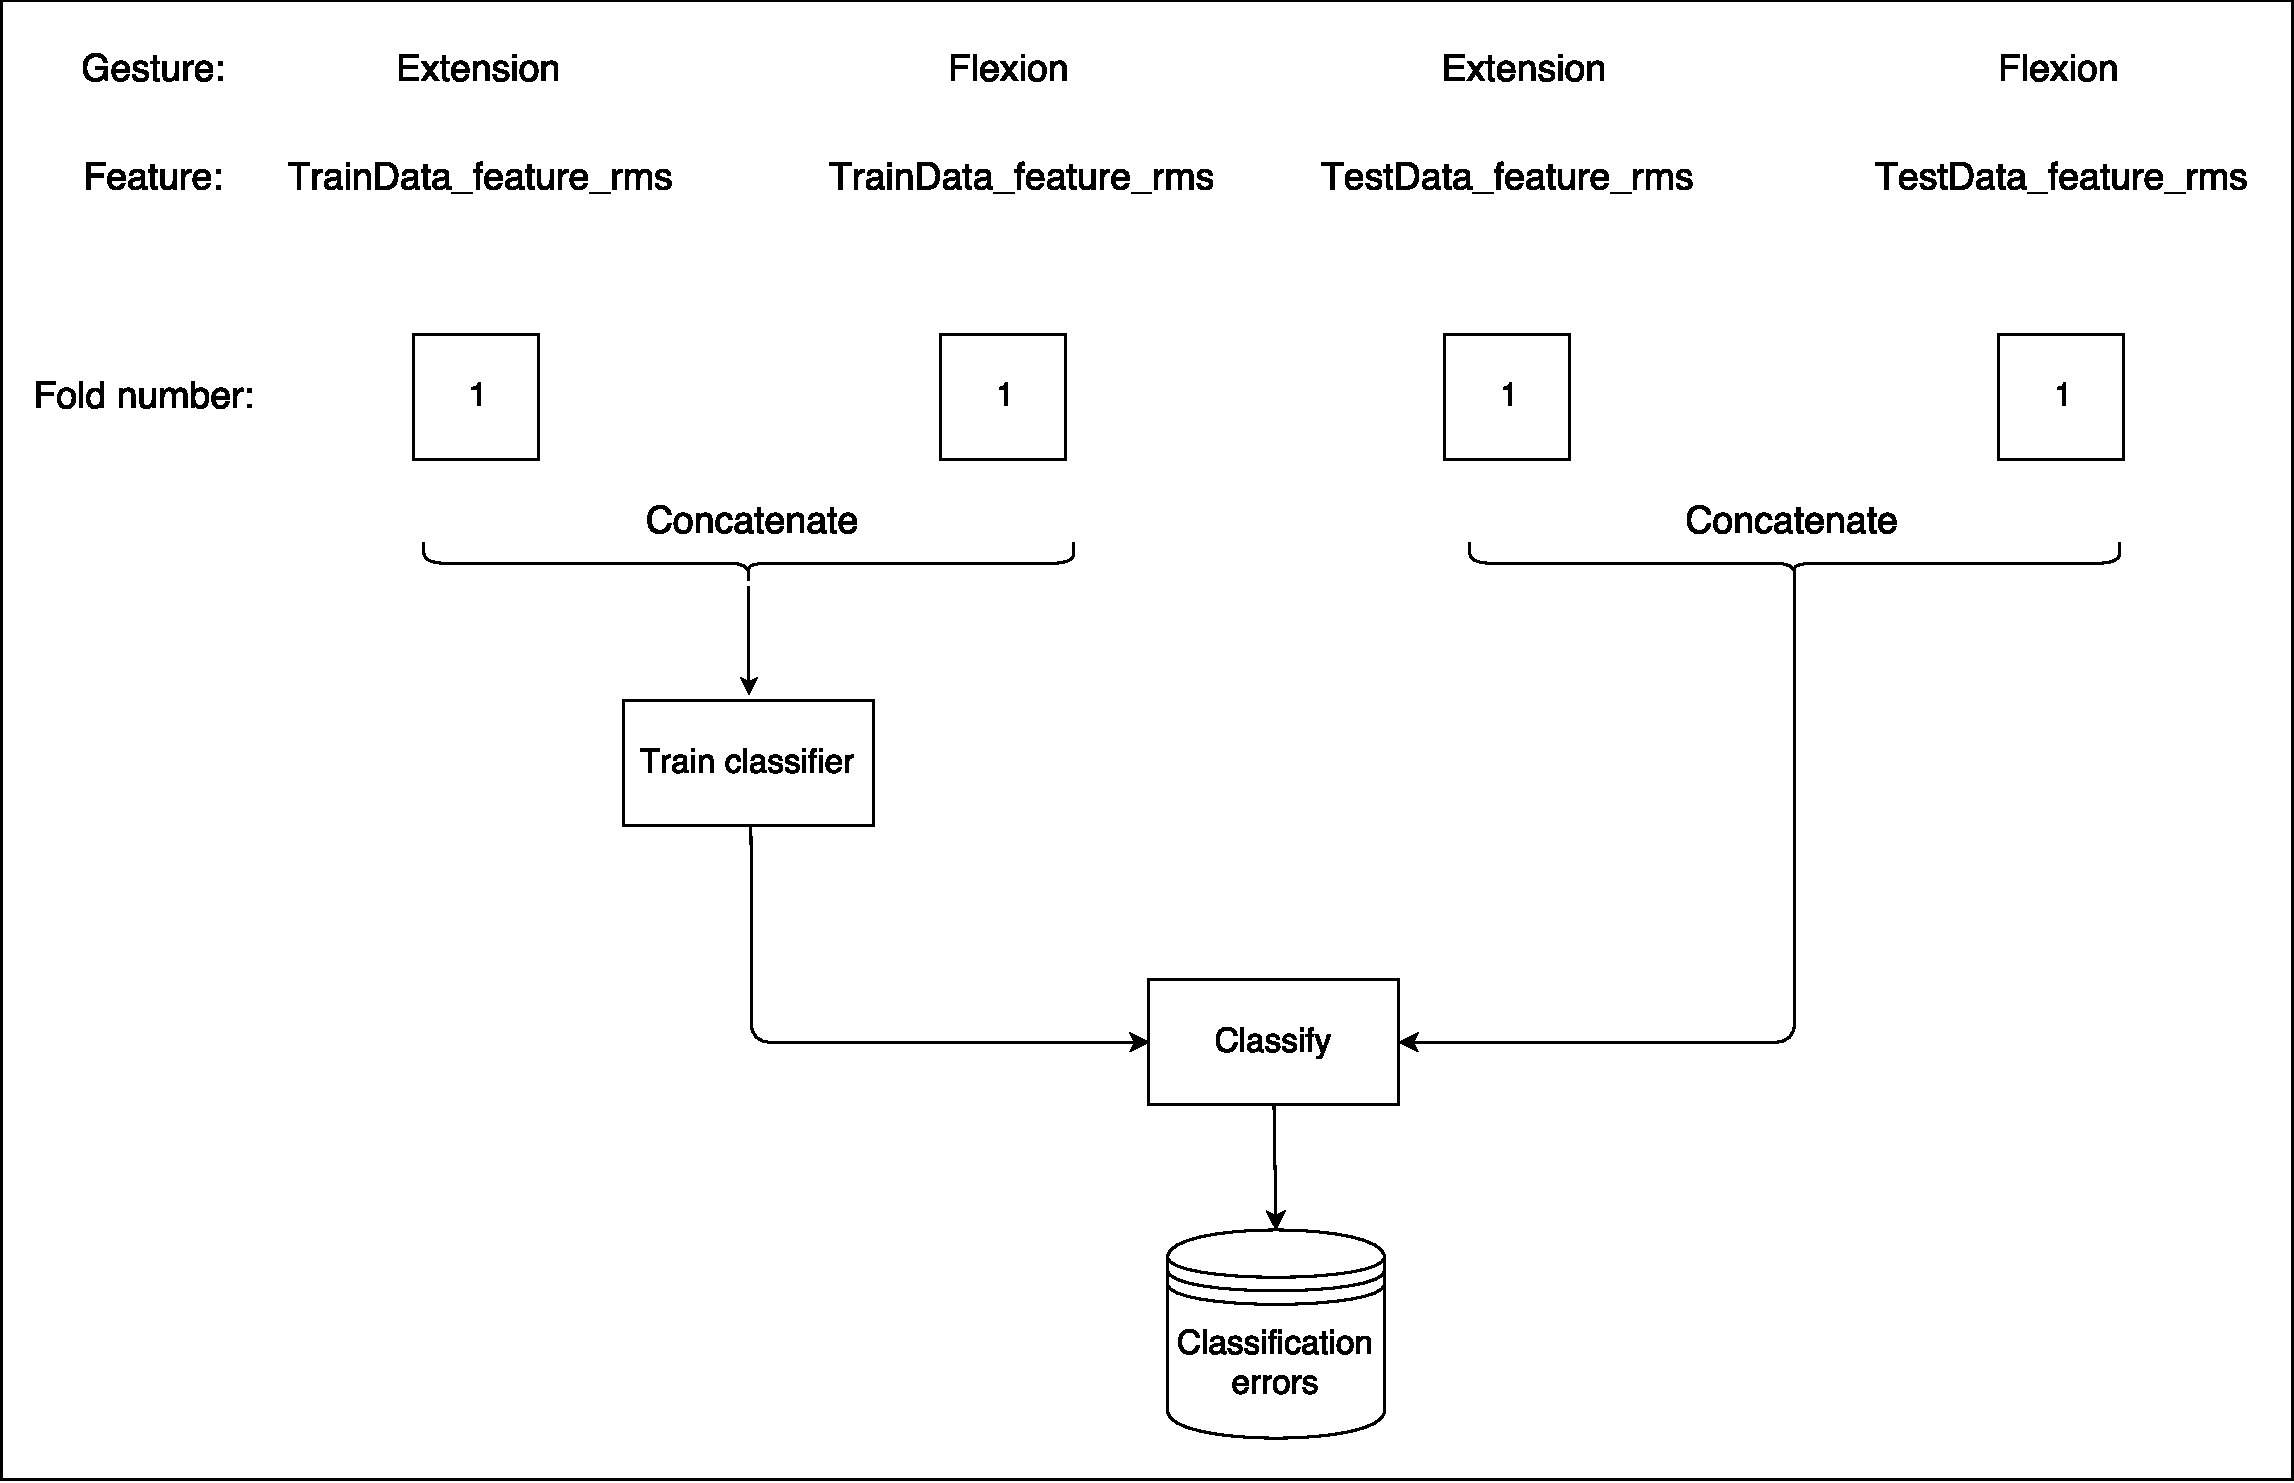
\includegraphics[width=15cm,center,keepaspectratio]{figures/train_classification}
\caption{Training \& classification: For the training part we concatenate the n-th training fold with the extension and the flexion data for each of the extracted features. We proceed by training the model with these data. Then, we concatenate the n-th test fold for the extension and flexion data and for the same feature as we did for the training folds. After testing the newly trained neural network with the test data we have the detection accuracies. }
\label{fig:train_classification}
\end{figure}
\subsection{Forward selection, backward elimination}
A common problem in pattern classification is to select a subset of features from a pool of many potential variables. As in most cases, in ours too, data acquisition process collects samples on a large number of variables because it is unknown which ones are the most important for class discrimination. To identify and select the most important and nonredundant variables from the large pool of potential variables is the goal of the feature subset selection \cite{mao_orthogonal_2004}.\\
In the work of Jovic et al. forward selection typically starts with an empty feature set and then considers adding one or more features to the set \cite{jovic_review_2015}.\\
In backward elimination, we typically start with the whole feature set and considers removing one or more features from the set.\\
Bidirectional search start from both sides, from an empty set and from the whole set, simultaneously considering larger and smaller feature subsets. Heuristic selection generates a starting subset based on a heuristic and then explores it further.\\
\section{Artificial intelligence}
Artificial intelligence (\ac{AI}) is a thriving field with many practical applications and current active research topics. AI tries to automate routine labor, understand speech or images, make diagnoses in medicine and support scientific research with the creation of intelligent software \cite{Goodfellow-et-al-2016}.\\
Artificial intelligence rapidly tackled and solved problems that are difficult for human beings but relatively straight-forward for computers, problems that can be described by a list of mathematical formulas. The demanding challenge for artificial intelligence is to solve tasks that are easy for people to solve but hard for them to describe formally, problems that we solve intuitively such as recognizing faces \cite{Goodfellow-et-al-2016}.\\
Computers have been able to defeat the best human chess players but only recently to recognize object or speech. A life of a person demands an immense amount of world knowledge. Much of this knowledge is subjective and therefore difficult to formally articulate. Thus, one of the key challenges in artificial intelligence is how to transfer this informal knowledge into the computer \cite{Goodfellow-et-al-2016}.\\
One solution is to create a knowledge base where we have to hard-code knowledge about the world formally. That will make the computer able to reason automatically about statements in languages that are designed to be used with logical inference rules. The disadvantage is that people struggle to describe everything about the world formally with logical rules \cite{Goodfellow-et-al-2016}.\\
This main disadvantage suggest that AI systems need the ability to acquire their own knowledge, by extracting patterns from data. This capability is also known as \textbf{machine learning}. The introduction of machine learning enable the computers to overcome problems that require knowledge of the real world and make decisions that appear subjective\cite{Goodfellow-et-al-2016}.\\
Many artificial intelligence  tasks can be solved by finding the right set of features to extract for that task, then providing these features to a simple machine learning algorithm such as logistic regression or naive Bayes. Although, for many tasks, is difficult to know what features should be extracted. \\
A way to improve machine learning with feature extraction is to use machine learning to discover the representation itself. This is known as representation learning. With this approach, the AI systems are enabled to adapt to new tasks faster with minimal human intervention. A representation learning algorithm can discover a good set of features for a complex task requires hours to months whereas the same complex task would require a great deal of time and effort.
\subsection{Biological and artificial neural networks}
The human brain is the most complex and most powerful organ of the human body. The inner functionality of the human brain is modeled around the \textit{neurons} and the networks of neurons known as \textit{biological neural networks}. The estimated number of human brain neurons is 100 billion, which are interconnected and communicate with one another through an interface consisting of \textit{axon terminals} that are connected to \textit{dendrites} across a gap (synapse) as shown in Fig. \ref{fig:biological_neuron}. 
\begin{figure}[h!]
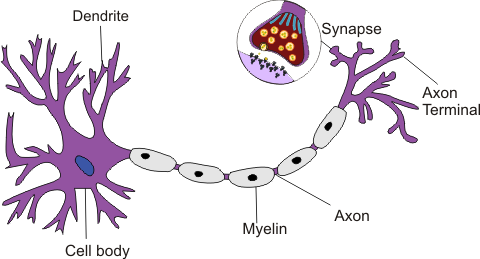
\includegraphics[width=10cm,center,keepaspectratio]{figures/biological_neuron}
\caption{Anatomy of a biological neuron \cite{fig:biological_neuron}}
\label{fig:biological_neuron}
\end{figure}
Simply put, the neuron will pass a message to another neuron across this interface if the sum of weighted input signals from one or more neurons exceeds a threshold to cause the message transmission. When the threshold is exceeded and the message is passed along to the next neuron is known as \textit{activation}.\\
An artificial neural network is basically a mathematical function. It is built from simple functions which have parameters which get adjusted. An example of such a function is shown in Fig. \ref{fig:artificial_neuron}. The below network takes $x_1$ to $x_n$ as numerical inputs and has weights $w_1$ to $w_n$ associated with these inputs. Additionally, there is another input $1$ with bias $b$ (called the bias) associated with it. There are thousands of those simple functions (also called ``neurons'') which build an artificial neural network. Each neuron's input signal is a weighted combination of many input signals and the weight of each input means that the input can have a different influence  on any subsequent calculations, und ultimately on the final output of the entire network. In addition, the main function of bias is to provide every node with a trainable constant value in addition to the normal inputs that the node receives. \\
\begin{figure}[h!]
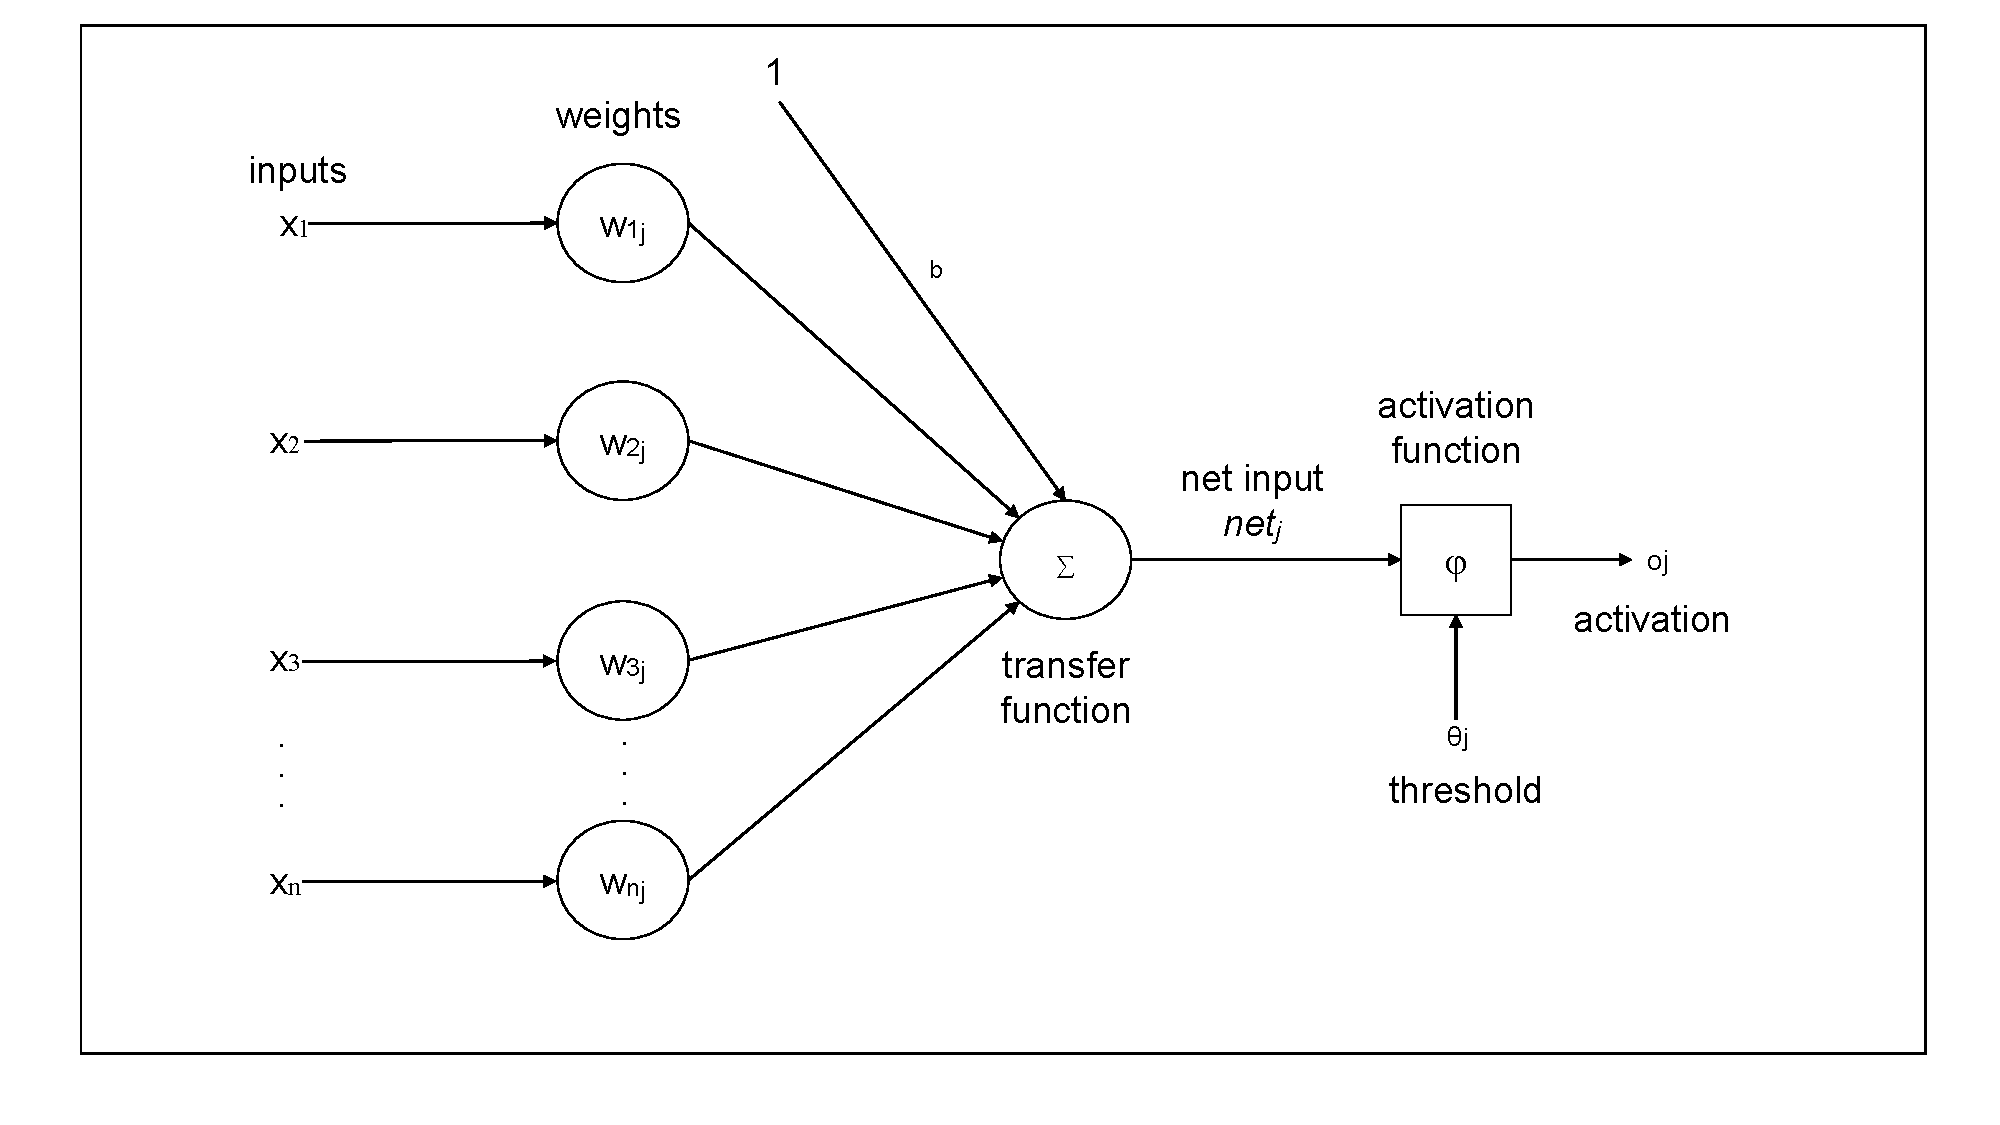
\includegraphics[width=15cm,center,keepaspectratio]{figures/artificial_neuron}
\caption{Artificial neuron}
\label{fig:artificial_neuron}
\end{figure}
Additionally, each neuron applies a transformation function to the weighted inputs, meaning that the summed weighted input signal is transformed mathematically prior to evaluating only if the activation threshold is exceeded. Here we list some of the several activation functions someone can encounter in practice: log-sigmoid, tan-sigmoid, the positive linear often referred to as rectified linear unit (ReLU) and the softmax tranfer functions which we will explain them later in detail. The combination of the weighted of input signals and the functions applied are typically either linear or nonlinear.\\
These input signals can originate in many ways, with our senses being some of the most important, as well as breathing, drinking and eating for example. A single neuron can receive hundreds of thousands of these input signals at once that undergo the summation process to determine if the message gets passed along and ultimately causes the brain to instruct actions, memory recollection and so on.\\
All the thoughts which are generated in our brains and the subsequent instructions given to our muscles, organs, and body are the results of these neural networks in action. The brain's neural networks continuously change and update themselves in many ways, including modifications to the amount of weighting applied among the neurons.\\
Ergo, it comes naturally to assume that, in order to transfer the brain's functionality and capabilities to  a computing machine, it must be implemented by a computer, artificial version of this network of neurons. This is the birth of this statistical processor and  known as \textit{artificial neural networks}. \\
\subsection{Artificial neural networks}
Artificial neural network is an interconnected group of natural or artificial neurons that uses a mathematical or computational model inspired by and modeled on biological neural networks. They are capable of processing nonlinear relationships between inputs and outputs in parallel. These networks are characterized by containing adaptive weights along the paths of many neurons which can be tuned by a learning algorithm which learns from observed data in order to improve the model. Apart from the learning algorithm, a cost function has to be chosen.\\
The cost function is used to learn the optimal solution to the problem being solved. It helps in determining the best values for all the tunable parameters, by adapting the weights along with other parameters such as the learning rate. These values are determined through optimization techniques such as gradient descent or stochastic gradient descent. These optimization techniques try to find the optimal solution, which when successful that means that ANN is able to solve the problem in question with a high accuracy. \\
Architecturally, an artificial neural network is modeled using layers  of artificial neurons, as shown in Fig. \ref{fig:artificial_neuron}, which are able to receive input and apply an activation function along with a threshold to determine if messages are passed along.\\
As shown in Fig. \ref{fig:simple_neural_network} the first layer in a neural network model is always the input layer followed by one hidden layer and lastly by an output layer. Each layer can contain one or more neurons. Models become increasingly complex by increasing the number of hidden layers, the number of neurons in any given layer or the number of paths between neurons. The following network is also known as feed-forward network. \\
\begin{figure}[h!]
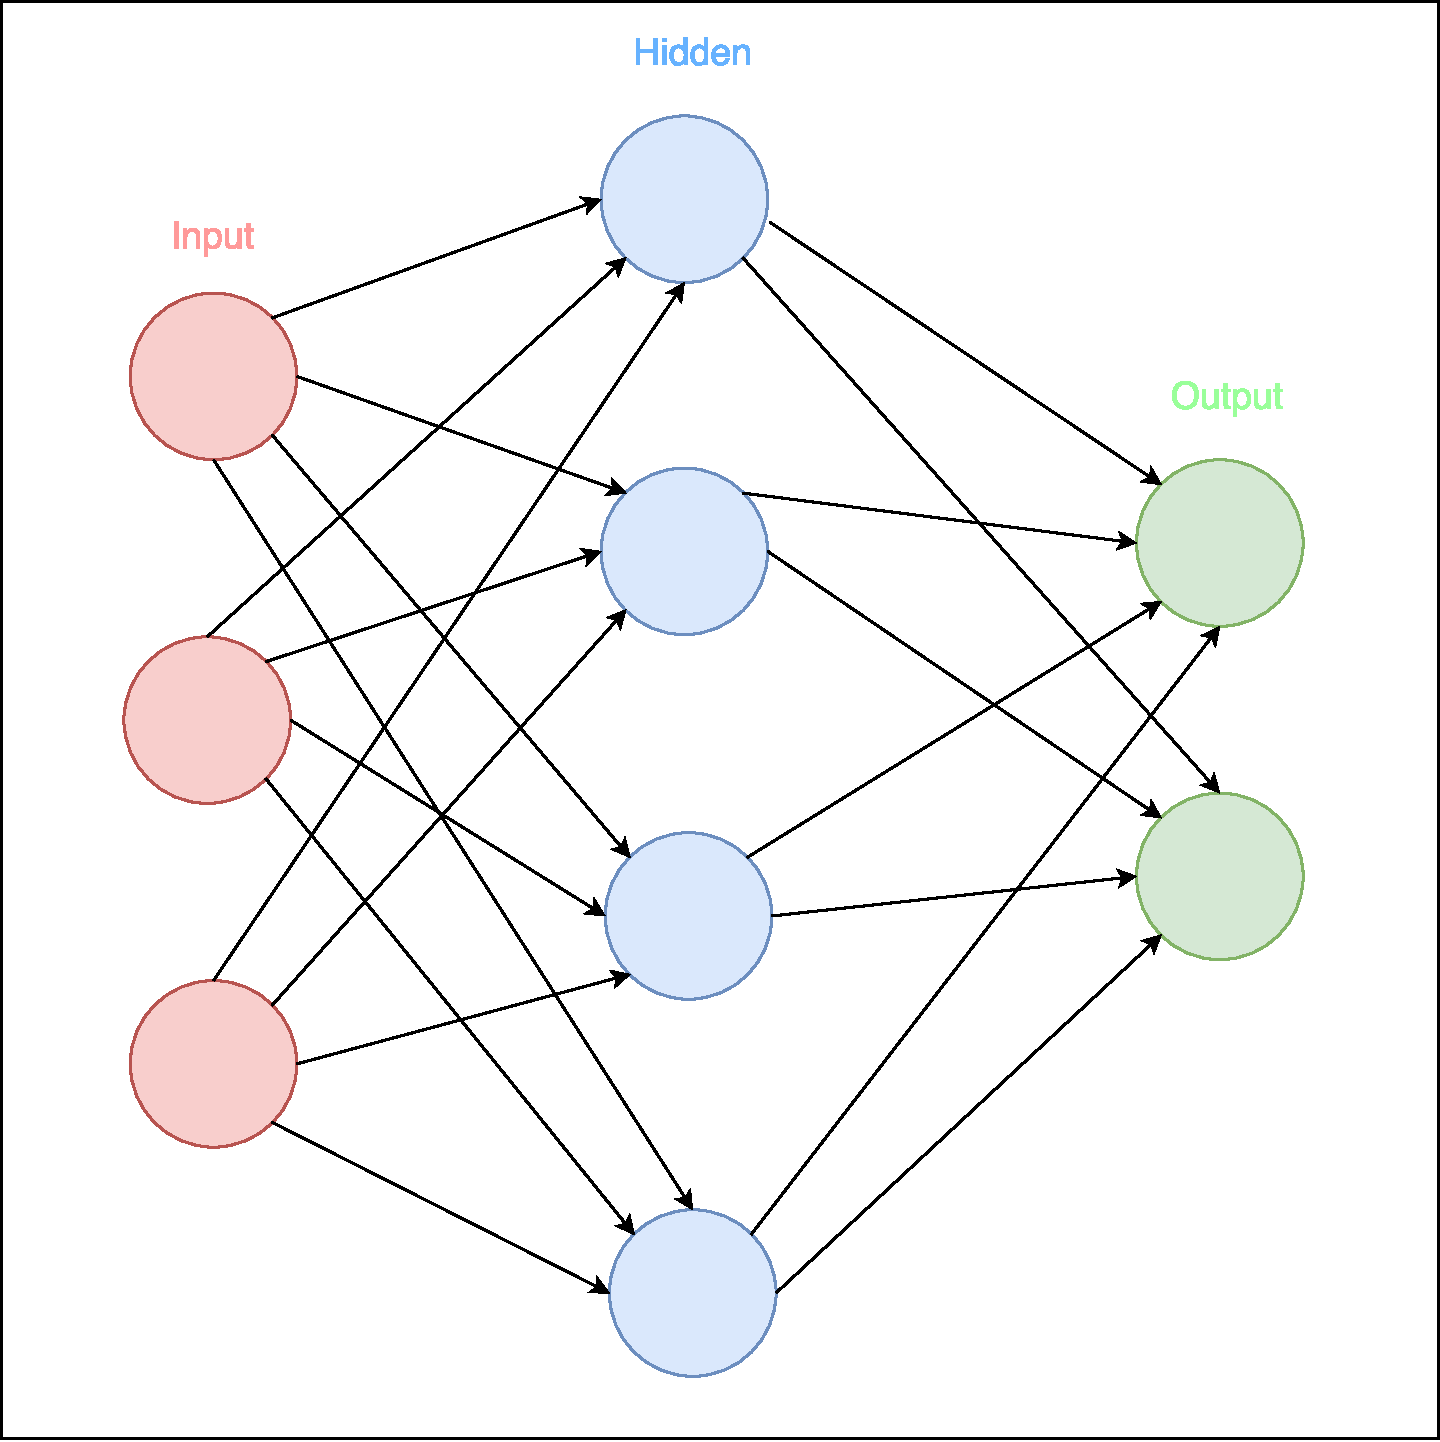
\includegraphics[width=10cm,center,keepaspectratio]{figures/simple_neural_network}
\caption{Feed-forward network}
\label{fig:simple_neural_network}
\end{figure}
Model architecture and tuning are therefore major components of ANN techniques in addition to the learning algorithms themselves. All of these characteristics of an ANN can have significant impact on the performance of the model.In addition, models are tuned by the activation function to convert a neuron's input to its output activation. \\
The meaning represented by a single artificial neuron is a form of local representation whereas the meaning of the entire neural network is a form of a distributed representation  due to the accumulated transformations across the neurons and layers.
\subsection{Deep learning}
Many machine-learning systems nowadays make an extended use of a class of techniques called deep learning. Deep learning also known as deep structured learning, is a branch of machine learning based on a set of algorithms that attempt to model high level abstractions in data. In a simple single-layer network we could have two sets of neurons: ones that receive an input signal and ones that send  an output signal. When the input layer receives an input it passes on a modified version of the input to the next layer. In a deep network, there are many layers between the input and the output, allowing the algorithm to use multiple processing layers, composed of multiple linear and non-linear transformations. \cite{Goodfellow-et-al-2016}\\
These methods have improved the state-of-the-art in speech recognition \cite{hinton_deep_2012}, object recognition \cite{girshick_rich_2014} and in other domains such as drug discovery \cite{gawehn_deep_2016} and genomics \cite{park_deep_2015}. The term ``Deep Learning'' was first introduced to machine learning by Dechter \cite{dechter_learning_1986}.
\subsection{Deep learning architecture}
We are going to list briefly the different deep learning architectures:
\begin{itemize}
\item \textbf{Generative deep architectures}, which are intended to characterize the high-order correlation of the observed or visible data for pattern analysis and characterize the joint statistical distributions of the visible data and their associated classes. \cite{dechter_learning_1986} Some of the types of generative models are hidden markov model and restricted boltzmann machine.
\item \textbf{Discriminative deep architectures}, which are intended to directly provide discriminative power for pattern classification, often by characterizing the posterior distributions of classes conditioned on the visible data. Some types of discriminative architecture are support vector machines, logistic regression which is a type of generalized of linear regression which is used for predicting binary or categorical outputs. 
\item \textbf{Hybrid deep architectures}, where the goal is discrimination but is assisted with the outcomes of generative architectures via better optimization and regularization, or discriminative criteria are used to learn the parameters in any of the deep generative models is the generative deep architectures category. \cite{deng_three_2012}
\end{itemize}
\subsection{Deep feed forward networks}
Deep feed-forward networks, also called feed-forward neural networks, or multilayer perceptrons (\ac{MLP}), are the quintessential deep learning models.\\
The goal of a feed-forward network is to approximate some function f$^{*}$ . For example, for a classifier, $y = f ^{*} (x)$ maps an input $x$ to a category $y$. A feedforward network defines a mapping $y = f(x;\theta)$ and learns the values of the parameters $\theta$ that result in the best function approximation.\cite{Goodfellow-et-al-2016}\\
In simple terms, the network can be defined as input, hidden and output nodes with data coming in from input node, processing is done in hidden nodes and then the output is produced  through the output nodes. The information  flows through the function being evaluated from $x$, through the intermediate computations used to define $f$, and finally to the output $y$. There are no feedback connections in which outputs of the model are fed back into itself and hence the models is called as feed-forward network. When feedforward neural networks are extended to include feedback connections, they are called recurrent neural networks. These kind of networks are used in many natural language applications \cite{mikolov_recurrent_2010}. The convolutional networks which are used for object recognition from photos are a specialized kind of feedforward network.\cite{Goodfellow-et-al-2016} \\
Deep feedforward networks also called \textbf{feedforward neural networks} or multilayer perceptronsare the most important deep learning models. Feedforward neural networks are called networks because they are typically represented by  composing together many different functions \cite{Goodfellow-et-al-2016}. The model is associated with a directed acyclic graph describing how the functions are composed together. For example, we might have three functions $f^{(1)},f^{(2)}$ and $f^{(3)}$ connected in a chain, to form $f(x) = f^{(3)}(f^{(2)}(f^{(1)}(x)))$. These chain structures are the most commonly used structures of neural networks. In this case, $f^{(1)}$ is called the first layer of the network, $f^{(2)}$ is called the second layer, and so on. The overall length of the chain gives the depth of the model. The name ``deep learning'' arose from this terminology. The final layer of a feedforward  network  is called the output layer. During neural network training, we drive $f(x)$ to match $f^{*}(x)$. The training data evaluate $f(x)$ with noisy, approximate examples of $f^{*}(x)$ at different training points. Each example $x$ is accompanied by a label $y \approx f^{*}(x)$. The training examples specify directly what the output layer must do at each point $x$; it must produce a value that is close to $y$. The learning algorithm must decide how to use those layers to produce the desired output, but the training data do not determine what each individual layer is expected to do. Instead, the learning algorithm must decide  how to use these layers to best implement an approximation of $f^{*}(x)$. Because the training data does not show the desired output for each of these layers, they are called \textbf{hidden layers}. \cite{Goodfellow-et-al-2016}\\
As these networks are inspired by neuroscience these networks are called neural. Each hidden layer of the network is vector valued. The dimensionality of these hidden layers determines the width of the model. Each element of the vector can be interpreted as playing a role analogous to a neuron. Rather than thinking of the layers as representing a single vector-to-vector function, we can imagine the layer as consisting of many inputs that act in parallel, each representing a vector-to-scalar function. Each unit resembles a neuron in the sense that it receives input from many other units and computes its own activation value. The idea of using many layers of vector-valued representations is originating from neuroscience.  The choice of the functions $f^{(i)}(x)$ used to compute these representations is also guided by neuroscientific observations about the functions that biological neurons compute. It is best to think of feedforward networks as machines that try to approximate functions which are designed to achieve statistical generalization.  \cite{Goodfellow-et-al-2016}\\
Linear models can help us to find a way to understand feedforward networks. Linear models such as logistic regression and linear regression, are appealing  because they can be fit efficiently and reliably. Linear models also have the obvious defect that the model is limited to linear functions, so the model cannot understand the interaction between any two input variables. \\
To represent nonlinear functions of $x$, we can apply the linear model not to $x$ itself but to a transformed input $\phi(x)$, where $\phi$ is a nonlinear transformation. We can think of $\phi$ as providing a set of features describing $x$, or as providing a new representation for $x$. 
The question arises on how to choose the mapping $\phi$.
\begin{itemize}
\item One option is to use a generic $\phi$. If $\phi(x)$ has high dimension, we can have enough capacity to fit the training set, but generalization to the test set remains poor. Very generic feature mappings are usually based only on the principal of local smoothness and do not encode enough prior information to solve advanced problems. \cite{Goodfellow-et-al-2016}
\item Another way is to manually configure $\phi$. Till the advent of deep learning, this was the dominant approach. It requires a lot of human effort for each separate task, with practicioners in different domains, such as speech recognition of computer vision.\cite{Goodfellow-et-al-2016}
\item The strategy of deep learning is to learn $\phi$. In this approach, we have a model $y = f(x;\theta,w)= \phi(x;\theta)^T w $. $\theta$ parameter is used to learn $\phi$ from a broad class of functions, and parameter $w$ that map from $\phi(x)$ to the desired output. This is an example of a deep feedforward network, with $\phi$ defining a hidden layer. In this approach, we parameterize the representation as $\phi(x;\theta)$ and use the optimization algorithm to find the $\theta$ that corresponds to a good representation. The advantage with this approach is that the human designer only needs to find the right general function family rather than finding precisely the right function.  \cite{Goodfellow-et-al-2016}\\
\end{itemize}
The general principle of improving models by learning features extends beyond the feedforward networks. Feedforward networks are the application of this principle to learnings deterministic mapping from $x$ to $y$ that lack feedback connections. Other models, apply these principles to learning stochastic mappings, functions with feedback and probability distributions over a single vector. \cite{Goodfellow-et-al-2016}\\
Last but not least, feedforward networks have introduced the concept of hidden layer, and this requires us to choose the activation functions that will determine the hidden layer values. We should also take into consideration about how many layers the network should contain, how these layers should be connected to each other and how many units should be in each layer. Learning in deep neural networks requires computing the gradients of complicated functions. The back-propagation is one of these algorithms which are used to compute these gradients. 
\subsection{Learning Conditional Statistics}
Instead of learning a full probability distribution $p(y |x;\theta)$, we want to learn just one conditional statistic of $y$ given $x$. For example, we may have a predictor $f(x;\theta)$ that we wish to employ to predict the mean of $y$. From this point of view, we can view the cost function as being a functional rather than just a function. A functional is a mapping from functions to real numbers. Therefore, we can think of learning as choosing a function rather than merely choosing a set of parameters. For example, we can design the cost functional to have its minimum lie on the function that maps $x$ to the expected value of $y$ given $x$. To solve the optimization problem with respect to a function requires a mathematical tool called \textbf{calculus of variations}. \cite{gelfand_calculus_2000}
Our first result derived using calculus of variations is that solving the optimization problem
\begin{equation}
f^{*} = argmin \mathbb{E}_{x,y \sim p_{data}}||y - f(x)||^2
\end{equation}
yields
\begin{equation}
f^*(x) = \mathbb{E}_{y \sim p_{data}(y|x)}[y] 
\end{equation}
so long as this function lies within the class we optimize over. To put it simply, if we could train on infinitely many samples from the true data generating distribution, minimizing the mean squared error cost function would give a function that predicts the mean of $y$ for each value of $x$.\\
Different cost functions give different statistics. A second result derived using calculus of variations is that:
\begin{equation}
f^* = arg min \mathbb{E}_{x,y \sim p_{data}}
\end{equation}
yields a function that predicts the median values of $y$ for each $x$, as long as such a function may be described by the family of functions we optimize over. This cost function is commonly called \textbf{mean absolute error}.\cite{Goodfellow-et-al-2016}\\
\subsection{Common Activation Functions}
When we construct an ANN model, on of the main consideration is to choose the proper activation function for hidden and output layers that are differentiable. The main reason behind that, is that when we calculate the backpropagated error signal that is used to determine ANN parameter updates requires the gradient of the activation function gradient. Four of the most common functions and their associated gradients are plotted in Fig.\ref{fig:activation_functions} :
\begin{figure}[h!]
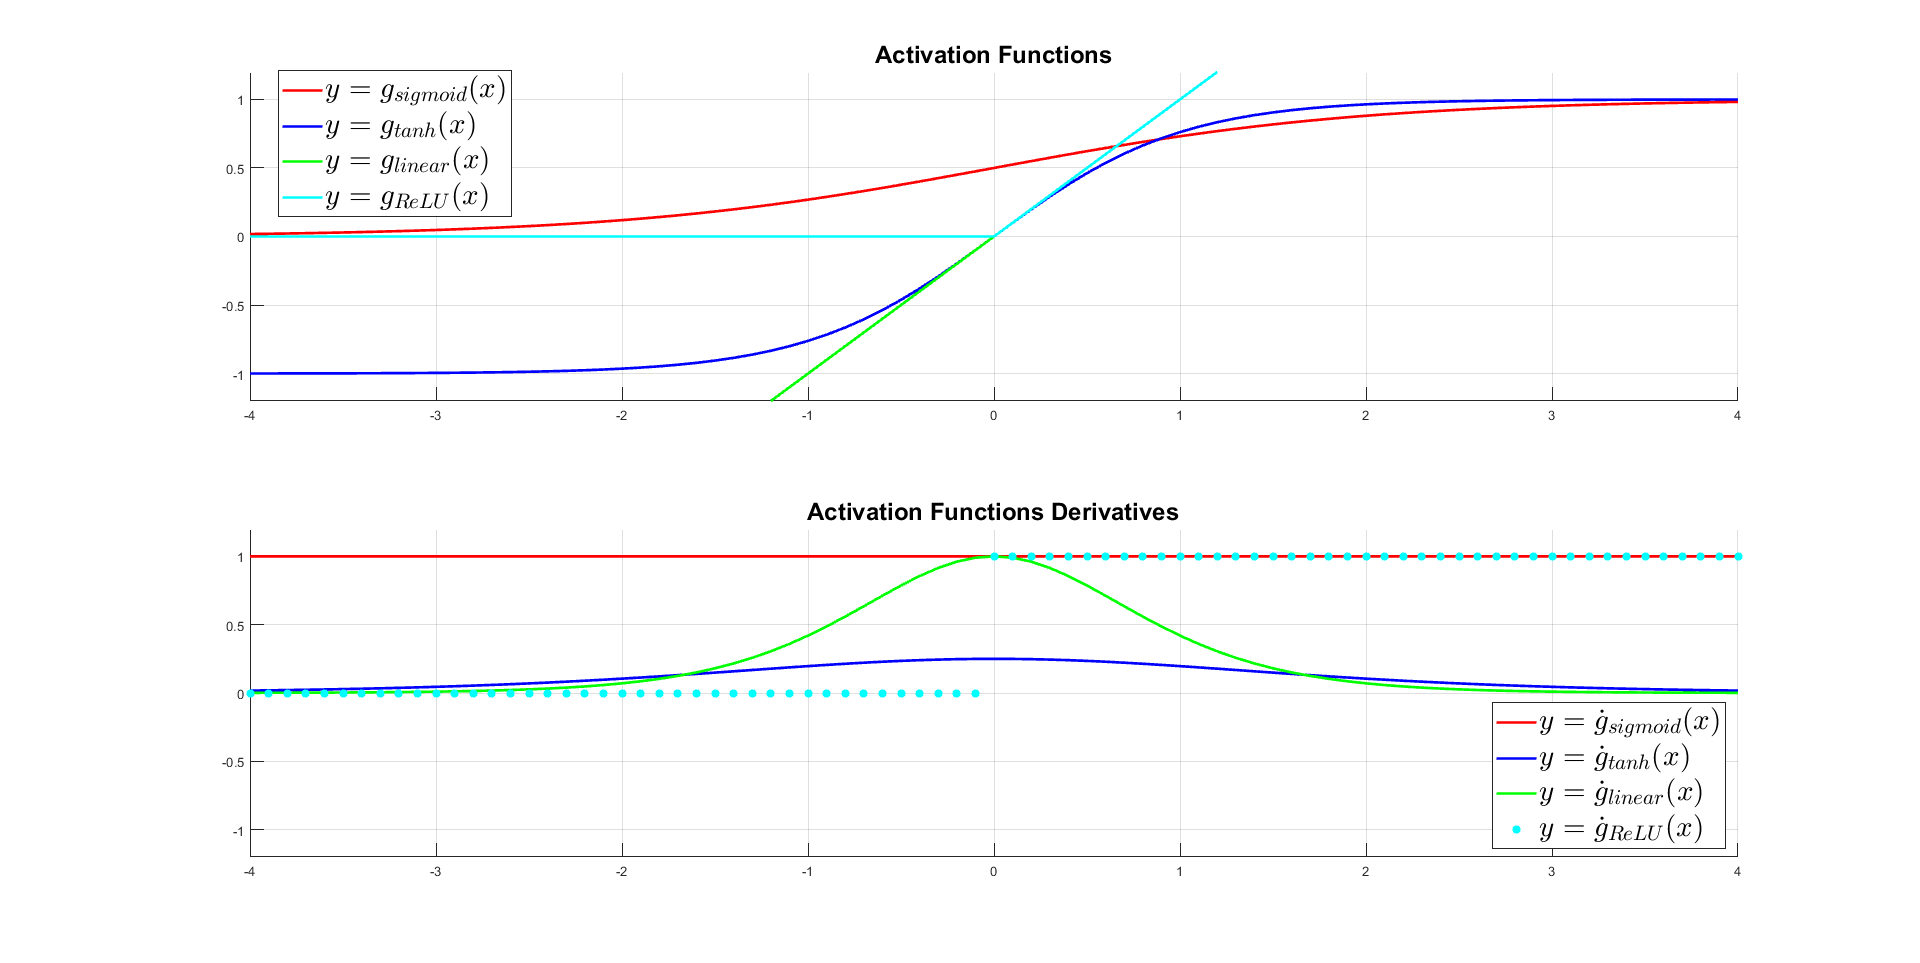
\includegraphics[width=20cm,center,keepaspectratio]{figures/activation_functions}
\caption{Common activation functions used in artificial neural networks along with their derivatives.}
\label{fig:activation_functions}
\end{figure}
\subsection{Identity Activation Function}
The simplest activation function, that is commonly used for the output layer in regression problems, is the identity/linear activation function:
\begin{equation*}
g_{linear}(z) = z
\end{equation*}
This activation function maps the pre-activation to itself and can output values that range $(-\infty,\infty)$. Even though, a multi-layered network with linear activations at each layer can be equally formulated as a single-layered linear network, the identity activation function seems to be extremely useful. In the case, where a multi-layered network that has nonlinear activations functions amongst the hidden units and an output layer  that uses the identity activation function implements a powerful form of nonlinear regression. \cite{Goodfellow-et-al-2016}
\subsection{Logistic Sigmoid}
A function that is often used as the output activation function for binary classification problems is the logistic sigmoid. The logistic sigmoid has the following form:
\begin{equation}
g(z) = \sigma (z) = \frac{1}{1 + \mathrm{e}^{-z}}
\end{equation}
and output values that range $(0,1)$. The logistic sigmoid can be interpreted as the probability of an artificial neuron ``firing'' given its inputs. Calculating the derivative of the logistic sigmoid makes use of the quotient rule:
\begin{equation}
\begin{split}
g'_{logistic} &= \frac{\partial}{\partial z}(\frac{1}{1+\mathrm{e}^{-z}})\\
          &= \frac{\mathrm{e}^{-z}}{(1+\mathrm{e}^{-z})^2}\\
          &= \frac{1 + \mathrm{e}^{-z} -1}{(1+\mathrm{e}^{-z})^2} \\
          &= \frac{1 + \mathrm{e}^{-z}}{(1+\mathrm{e}^{-z})^2} - (\frac{1}{1 + \mathrm{e}^{-z}})^2\\
          &= \frac{1}{(1+\mathrm{e}^{-z})} - (\frac{1}{1 + \mathrm{e}^{-z}})^2\\
          &= g_{logistic}(z) - g_{logistic}(z)^2\\
          &= g_{logistic}(z)(1 - g_{logistic}(z))
\end{split}
\end{equation}
This turns out to be convienient as we can see that $g'_{logistic}(z)$ evaluated at $z$ is $g_{logistic}(z)$ weighted by  $1-g_{logistic}(z)$ thus the gradients for the layers can be evaluated using simple multiplication and subtraction rather than performing any re-evaluating the sigmoid function, which requires extra exponentiation.\\
\subsection{Hyperbolic Tangent}
Although the logistic sigmoid has a biological interpretation, it turns out that the logistic sigmoid can cause a neural network to get ``stuck'' during training. In the case where a strongly-negative input is provided to the logistic sigmoid, it output values very near to zero. As we know, neural networks use the feedforward activations to calculate parameter gradients this affect the model parameters that are updated less regurarly than we would like and thus they are stuck in their current state.\cite{Goodfellow-et-al-2016} \\
An alternative to the logistic sigmoid is the hyperbolic tangent, or tanh function:
\begin{equation}
\begin{split}
g_{tanh}(z) &= \frac{sinh(z)}{cosh(z)}\\
			&= \frac{\mathrm{e}^z-\mathrm{e}^{-z}}{\mathrm{e}^z + \mathrm{e}^{-z}}
\end{split}
\end{equation}
As the logistic sigmoid, the tanh function is also sigmoidal but instead outputs values that range $(-1,1)$. Thus strongly negative inputs to the tanh will map to negative outputs. Additionally, zero-valued inputs are mapped to near-zero outputs. These properties make the network less likely to get ``stuck'' during training. Calculating the gradient for the tanh function also uses the quotient rule:
\begin{equation}
\begin{split}
g'_{tanh}(z) &= \frac{\partial}{\partial z}\frac{sinh(z)}{cosh(z)}\\
					&= \frac{\frac{\partial}{\partial z}sinh(z)cosh(z)-\frac{\partial}{\partial z}cosh(z)sinh(z)}{{cosh}^2(z)}\\
					&= \frac{{cosh}^2(z)-{sinh}^2(z)}{{cosh}^2(z)}\\
					&= 1 - \frac{{sinh}^2}{{cosh}^2}\\
					&= 1 - {tanh}^2(z)
\end{split}
\end{equation}
Similar to the derivative for the logistic sigmoid, the derivative of $g_{tanh}(z)$ is a function of feedforward activation evaluated at $z$, namely $(1 - g_{tanh}(z)^2)$.
\subsection{Rectified Linear Units}
Rectified linear units use the activation function $g(z) = max\{ 0,z \}$. These units are easy to optimize because they are similar to linear units. The only difference between a linear unit and a rectified linear unit is that a rectified linear unit outputs zero across half its domain. Therefore, this  makes the derivatives  through a rectified linear unit remain large whenever the unit is active. The gradients are not only large but also consistent. The second derivative of the rectifying operation is 0 almost everywhere, and the derivative of the rectifying operation is 1 everywhere the unit is active.\cite{Goodfellow-et-al-2016}\\
Rectified linear units are typically used on top of an affine transformation:
\begin{equation}
h = g(W^T x + b)
\end{equation}
When initializing the parameters of the affine transformation, it can be a good practice to set all elements  of b to a small positive value, such as 0.1. By doing so, it will be most likely that the rectified linear units will be active for most inputs in the training set and allow the derivatives to pass through. \\
When using a neural network to approximate a function, the data is forwarded through the network layer by layer until it reaches the final layer. The final layer's activations are the predictions that the network outputs. The essence of training our model  is to find the right set of weights for all the connections to make the right decision. To measure how well is our model performing we determine a metric which is also known as cost function. The discrepancies between the outputs in the estimations and the training set data are the principle values for our cost function. The goal of the training is to get the value of this cost function as low as possible.\cite{Goodfellow-et-al-2016}\\
\subsection{Softmax function}
The softmax transfer function is typically used as the transfer function for the output layer. It divides each output such that the total sum of the outputs is equal to one. The softmax function computes a categorical probability distribution that tells the probability that any of the classes are true. The mathematical formula for the softmax function is the following:
\begin{equation}
f{(z)}_i = \frac{e^{z_i}}{\sum_{j=1}^c e^{z}_j}
\end{equation}
In the above equation $z$ is a vector of the inputs to the output layer and $i$ indexes the output units.
\subsection{Minimization of the cost function}
One of the mostly used cost function is that of Mean-Squared-Error (\ac{MSE}) and we denote is as $J(W)$. 
\begin{equation}
J(W) = \frac{1}{m}\sum_{i=1}^m(h_W(x^{(i)})-y^{(i)})^2
\label{Eq:MSE_cost_function}
\end{equation}
where $m$ is the number of training examples, $x^{(i)}$ is the input vector for the $i^{th}$ training example and $y^{(i)}$ is the class label for the $i^{th}$ training example and $W$ are the chose parameter values or weights. Last but not least, $h_W(x^{(i)})$ is the algorithm's prediction for the $i^{th}$ training example using the parameters $W$.\cite{mccormickml}\\
We need to find the proper weights that will make the score of  this cost function as low as possible. Simply put we want to $\mathop{J(W)}_{\textbf{W}}$. To successfully minimize this function we need to take the first derivative and set it to zero and solve, which eventually will give us the locations of every minimum/maximum in this function. However, there are some difficulties with this approach:
\begin{itemize}
\item The cost function often is complex, so computing an expression for its derivative is time and resource consuming.
\item The cost function is also multi-dimensional and the need to find the points where all of those derivatives are zero is not trivial.
\item There is a large number of minima and maxima throughout the function and sorting out which one is the one we should be using is also computationally expensive. 
\end{itemize}
In addition to the aforementioned problems, as the size of networks begins to scale up, solving for the weights directly becomes increasingly infeasible. We overcome this problem by applying the so called iterative optimization algorithms which progressively work their way towards the optimal solution.\\
The most basic of the iterative optimization algorithms is the gradient descent. Generally, the cost function should be more or less convex, as Fig. \ref{fig:3D_convex_function} shows. To be truly convex however it is almost impossible. For the sake of simplicity, we need this example in order to explain how gradient descent works. \\
We start off by initializing our weight randomly, which puts us at the red as the Fig. \ref{fig:3D_convex_function} shows.
\begin{figure}[h!]
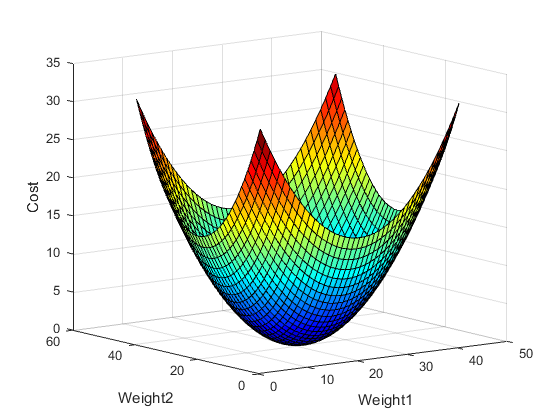
\includegraphics[width=10cm,center,keepaspectratio]{figures/3D_convex_function}
\caption{Convex function $z = x^2 + y^2$}
\label{fig:3D_convex_function}
\end{figure}
Taking the derivative, we see the slope at this point is a large positive number. Thus, we want to move closer to the center therefore we should take a large step in the opposite direction of the slope. If we repeat this process, eventually we will find the minimum of the curve as shown in Fig.\ref{fig:2D_convex_function} and much closer the optimal weight configuration for our model.
\begin{figure}[h!]
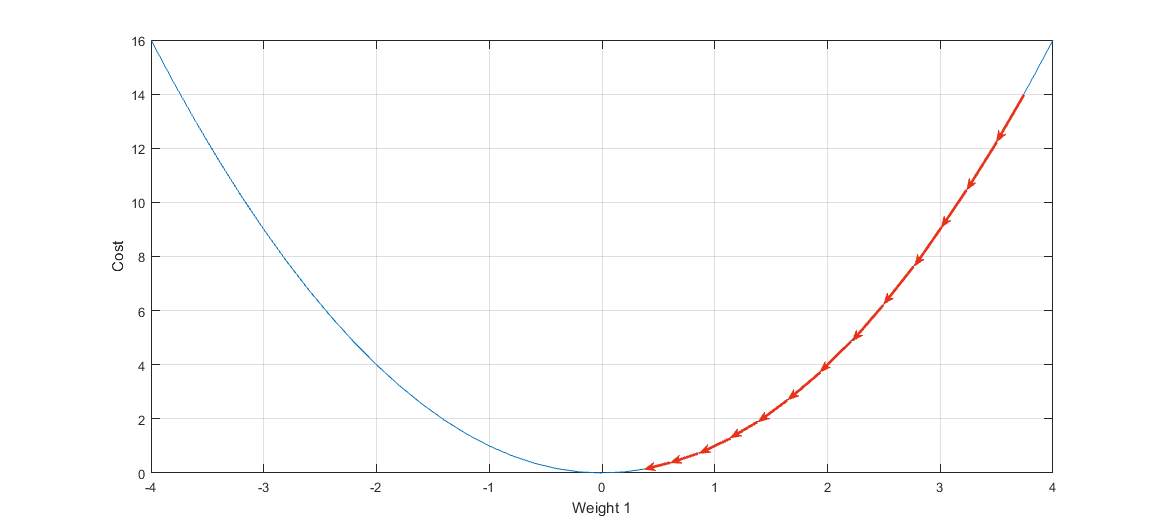
\includegraphics[width=16cm,center,keepaspectratio]{figures/2D_convex_function}
\caption{Convex function $y = x^2$}
\label{fig:2D_convex_function}
\end{figure}
The formula of gradient descent is as follows:
\begin{equation}
W := W - \alpha \frac{\partial J}{\partial W}
\end{equation}
where $\alpha$ is a parameter called  the learning rate. For example, we assume that we have as a cost function $J(W) = W^2$. We want to find the value of $W$ which minimizes $J(W)$. Let's assume that we start with $W=3$ and $\alpha = 0.1$. By doing simple calculations the Table \ref{table:gradient_descent_case} expresses how the value of $J'(W) = 2W$ changes and approaches to zero.
\begin{table}[h!]
\centering
{\rowcolors{2}{blue!10}{blue!20}
\renewcommand{\arraystretch}{1.3}
\begin{tabular}{ |p{2.5cm}|p{2.5cm}|p{2.5cm}|  }
\hline
Iteration & $W$ & $\alpha \frac{\partial J}{\partial W}$ \\
\hline
1 & 3     & 0.6 \\
2 & 2.4   & 0.48 \\
3 & 1.92  & 0.384 \\
4 & 1.536 & 0.307 \\
5 & 1.229 & 0.246 \\
6 & 0.983 & 0.197 \\
7 & 0.786 & 0.157 \\
8 & 0.629 & 0.126 \\
9 & 0.503 & 0.101 \\
10 & 0.403 & 0.081 \\
\hline
\end{tabular}
}
\caption{The values of W prior to each iteration and the update amounts.}
\label{table:gradient_descent_case}
\end{table}
As can be seen in our simple example, every time the weights are updated, there is a subtraction of the cost function with respect to the weight scaled by the learning rate $\alpha$. Thus, leads to the derivative term getting smaller and smaller and converging near to zero. Also, selecting the right learning rate is critical. If the learning rate is too large, we can overstep the minimum and diverge. On the contrary, if we choose a too small value for the learning rate we need to run more iteration of gradient descent and this will lead to the increase of the training tim \cite{mccormickml}.\\
In the above example we examined the case of a single variable cost function. Additionally to the single variable cost function we can have two or more variables in the cost function. Let's examine the case of the function $J(W) = W_1^2 + W_2^2$. This convex function is shown in Fig. \ref{fig:3D_convex_function}. When there are multiple variables in the minimization objective, gradient descent defines a separate update rule for each variable. Let's try to show mathematically how the derivatives of the cost functions build up:
\begin{align*}
\frac{\partial}{\partial W_1}J(W_1,W_2) = \frac{\partial}{\partial W_1}{W_1}^2 + \frac{\partial}{\partial W_1} {W_2}^2 = 2W_1 \\
\frac{\partial}{\partial W_2}J(W_1,W_2) = \frac{\partial}{\partial W_2}{W_1}^2 + \frac{\partial}{\partial W_2} {W_2}^2 = 2W_2
\end{align*}
As we can see, when we take the partial derivative with respect to $W_1$ we treat $W_2$ as a constant.\\
We showed the MSE cost function in Eq. \ref{Eq:MSE_cost_function}. Similarly, with the previous derivatives let's develop the derivative of the MSE cost function:
\begin{align*}
\frac{\partial}{\partial W_0}J(W_0,W_1) &= \frac{\partial}{\partial W_0}(\frac{1}{m}\sum_{i=1}^m (h_W(x^{(i)})-y^{(i)})^2)\\
&= \frac{1}{m}\sum_{i=1}^m \frac{\partial}{\partial W_0}(h_W(x^{(i)})-y^{(i)})^2)\\
&= \frac{1}{m}\sum_{i=1}^m 2(h_W(x^{(i)})-y^{(i)})\frac{\partial}{\partial W_0}(h_W(x^{(i)})-y^{(i)})\\
&= \frac{2}{m}\sum_{i=1}^m(h_W(x^{(i)})-y^{(i)})
\end{align*}
Lastly, each update of the $W$ variables is averaged over the training set. Every training example suggests its own modification to the weight values and then we average these suggestions to make our actual update. This means that the statistics of our training set are being taken into account during the learning process. An outlier training example (mislabeled or corrupted one) is going to have less influence over the final weights. \cite{mccormickml} \\
\subsection{Backpropagation}
Before the backpropagation algorithm there were many other methods implemented to adjust the weights in a random, uninformed direction (ie. increase or decrease) and check if the performance of the ANN is increasing. If it did not increase, then one would attempt to either go in the other direction or reduce the perturbation size or combine both \cite{ayearofai}.\\
Backpropagation give us an understanding on how to change the weights and biases in a network to have the desired changes on the cost function. For other machine learning algorithms like logistic regression (the sigmoid function) or linear regression computing the derivatives is an elementary application of differentiation. The same, however, cannot be said for neural networks. To demostrate this, we will demonstrate a diagram of a double-layered neural network:
\begin{figure}[h!]
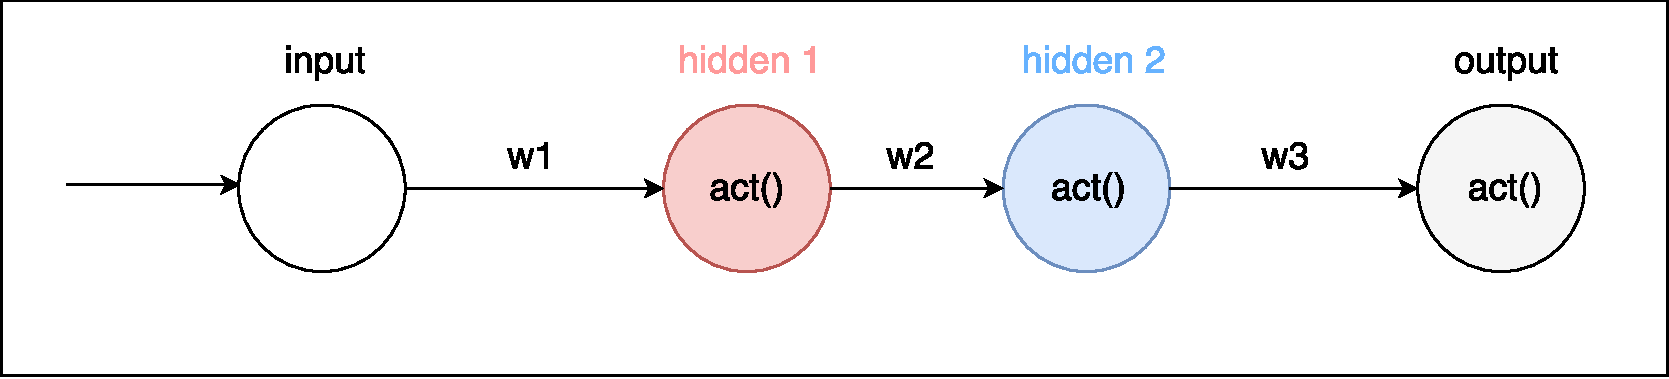
\includegraphics[width=15cm,center,keepaspectratio]{figures/double_layered_neural_network}
\caption{Double layered neural network}
\label{fig:double_layered_neural_network}
\end{figure}
In Fig. \ref{fig:double_layered_neural_network} we see that each neuron is dependent of the previous one connected to it. Put it simply, if we change the value of $w_1$, both ``hidden 1'' and ``hidden 2'' neurons (output layer inclusive) neurons will change. So we have the composite functions to compose the output function:
\begin{align*}
output &= act(w3 * hidden2)\\
hidden2 &= act(w2 * hidden1) \\
hidden1 &= act(w1 * input)
\end{align*}
Therefore we have:
\begin{equation}
output = act(w3 * act(w2*act(w1*input)))
\end{equation}
As we see, the output is a composite function of the weights, inputs and activation functions. Now, let's calculate the derivative  of this function with respect to the arbirtary weight for example $w1$. For this we have to apply the chain rule and we will have the following equation:
\begin{equation*}
\frac{\partial}{\partial w1}= \frac{\partial}{\partial hidden2}output* \frac{\partial}{\partial hidden1}hidden2 * \frac{\partial}{\partial w1}hidden1
\end{equation*}
If we are to compute the derivative of the error with any arbitrary weight the result equation will be:
\begin{equation*}
\frac{\partial error}{\partial w1}= \frac{\partial error}{\partial output}* \frac{\partial output}{\partial hidden2}* \frac{\partial hidden2}{\partial hidden1}*\frac{\partial hidden1}{\partial w1}
\end{equation*}
Each of these derivatives can be simplified once we choose an activation and error function as we discussed earlier. At this point, any abstraction has been removed, and the error derivative can be used in gradient descent to iteratively improve upon the weight. We compute the error derivatives according to every other weight in the network and apply gradient descent similarly. This procedure is called the backpropagation where the computation of the derivatives are fed to an optimization algorithm. The name backpropagation justifies the whole procedure as we are traversing from the output error to the weights, taking iterative steps using the chain rule until we reach the weight \cite{ayearofai}.\\
\subsection{Summary of training neural network}
We can summarize the steps of training an entire neural network:
\begin{enumerate}
\item Create our connected neural network and prepare training data
\item Initialize all the weights to random values. Here we have to emphasize we must not initialize the weights to zero. If weights are initialized to zero, the outgoing weights of each neuron will be identical because the gradients will be identical. Due to this, the proceeding hidden neurons will keep the same value and will continue to follow each other. This means that our neural network may get stuck at local optima. Therefore, random weight initialization allows us to overcome this problem by starting with many random values.\cite{ayearofai}
\item Perform one feed-forward using the training data
\item Perform backpropagation to get the error derivatives for each and every weight in the neural network
\item Perform gradient descent to update each weight of the respective error derivative.
\item If we have converged  training is complete. In reality most time, we stop when we have reached the number of maximum iterations. 
\end{enumerate}
\section{Data evaluation}
To test the optimal parameters for our neural network we need evaluation data. We created a new database with finger gestures consisted only from EMG signals. The signals were acquired with the Myo armband. The IMU data was discarded since there was no motion of the hand only motion of the fingers and keeping still the hand during the whole experiment. The 80\% percent of the new acquired data was used to train the neural nets and the rest 20\% was used to test the newly trained neural nets.\\
After the protocol for the new finger gestures was created and we created a database with the 14 new finger gestures and classify them into two classes: extension and flexion. We acquired new signals from the forearms of 21 subjects aged between 20-30. Below are the images with the extensions and the flexions of the gestures:
\begin{figure}
  \begin{subfigure}[t]{0.5\linewidth}
  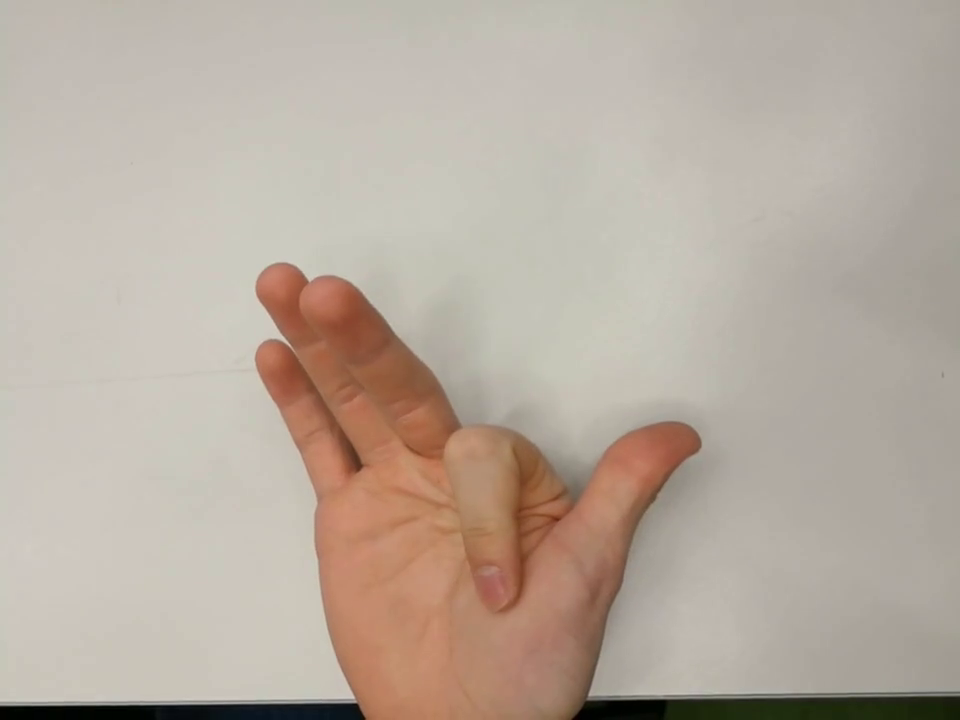
\includegraphics[width=100pt]{figures/ext_index1}
  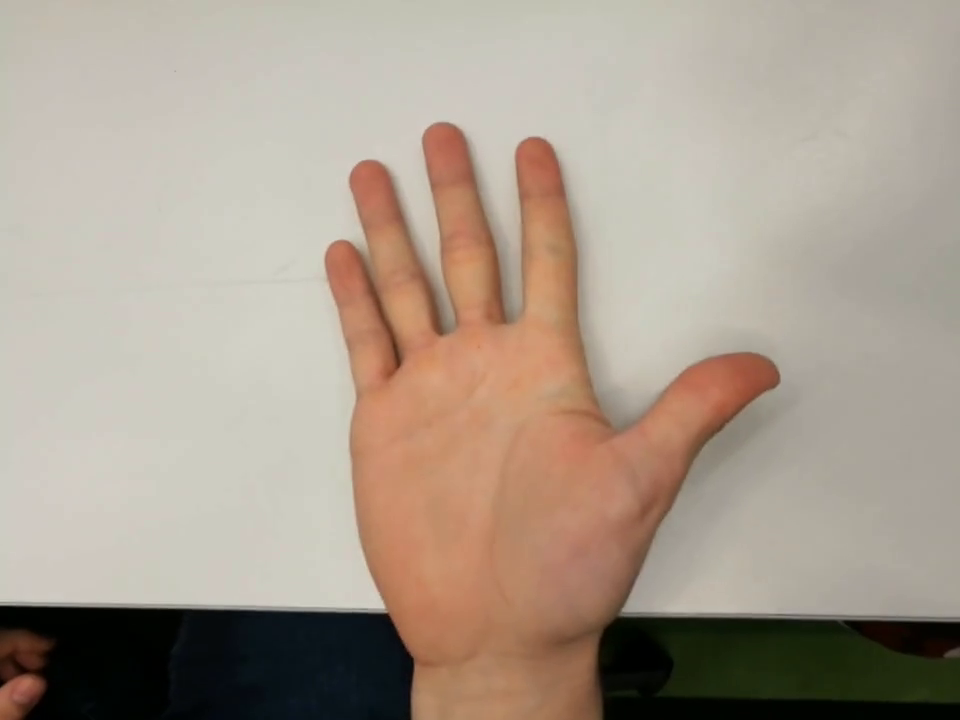
\includegraphics[width=100pt]{figures/flx_index1}
  \caption{G1: Index extension and flexion with the palm facing upwards}
  \end{subfigure}
  \hspace*{\fill}
  \begin{subfigure}[t]{0.5\linewidth}
  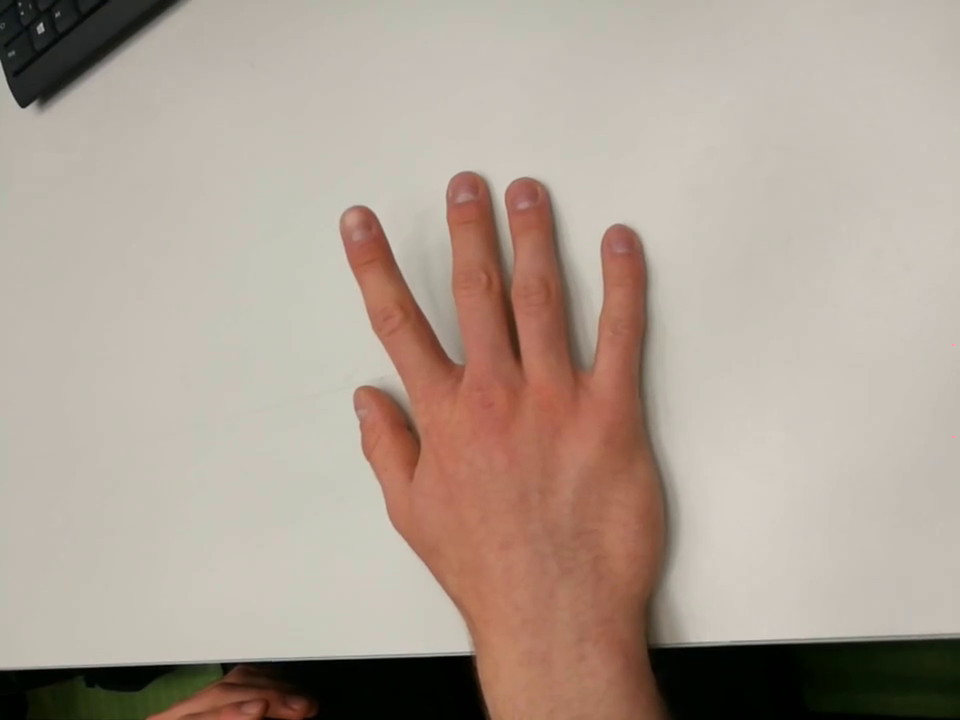
\includegraphics[width=100pt]{figures/ext_index2}
  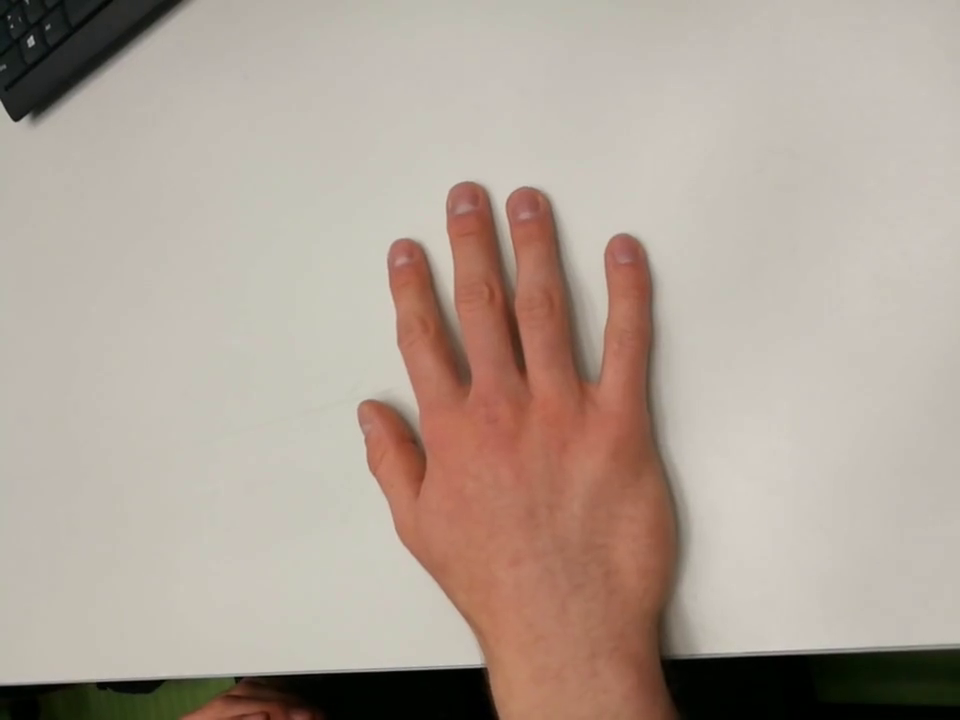
\includegraphics[width=100pt]{figures/flx_index2}
  \caption{G2: Index extension and flexion with the palm facing downwards}
  \end{subfigure}\par\medskip
  \begin{subfigure}[t]{0.5\linewidth}
  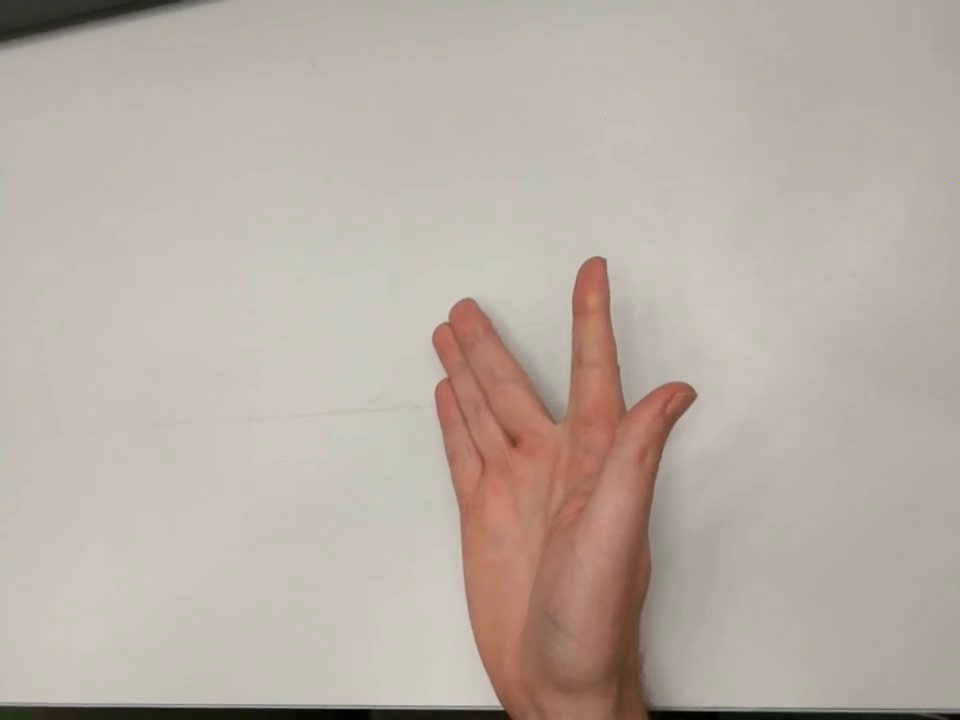
\includegraphics[width=100pt]{figures/ext_indextopair}
  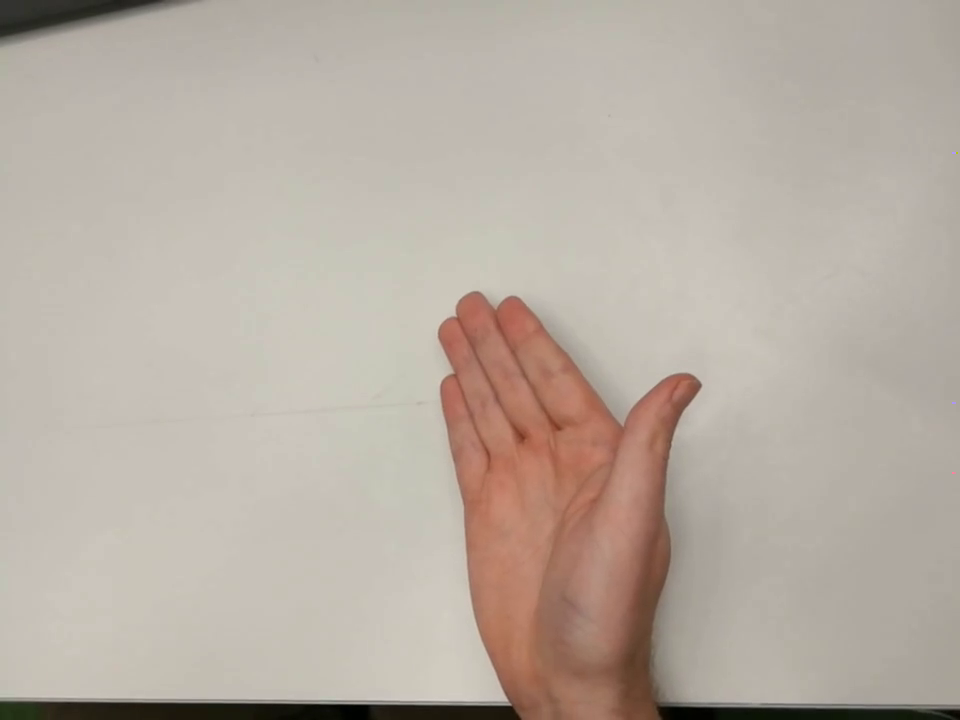
\includegraphics[width=100pt]{figures/flx_indextopair}
  \caption{G3: Moving index finger from and to pair(middle,ring,pinky)}
  \end{subfigure}
  \hspace*{\fill}
  \begin{subfigure}[t]{0.5\linewidth}
  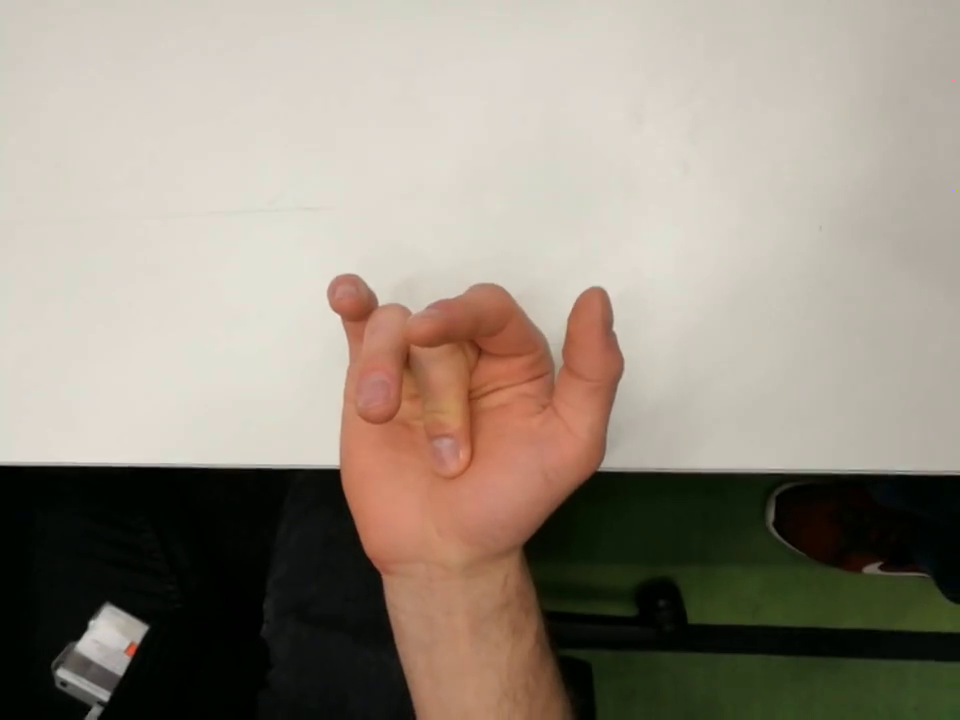
\includegraphics[width=100pt]{figures/ext_middle1}
  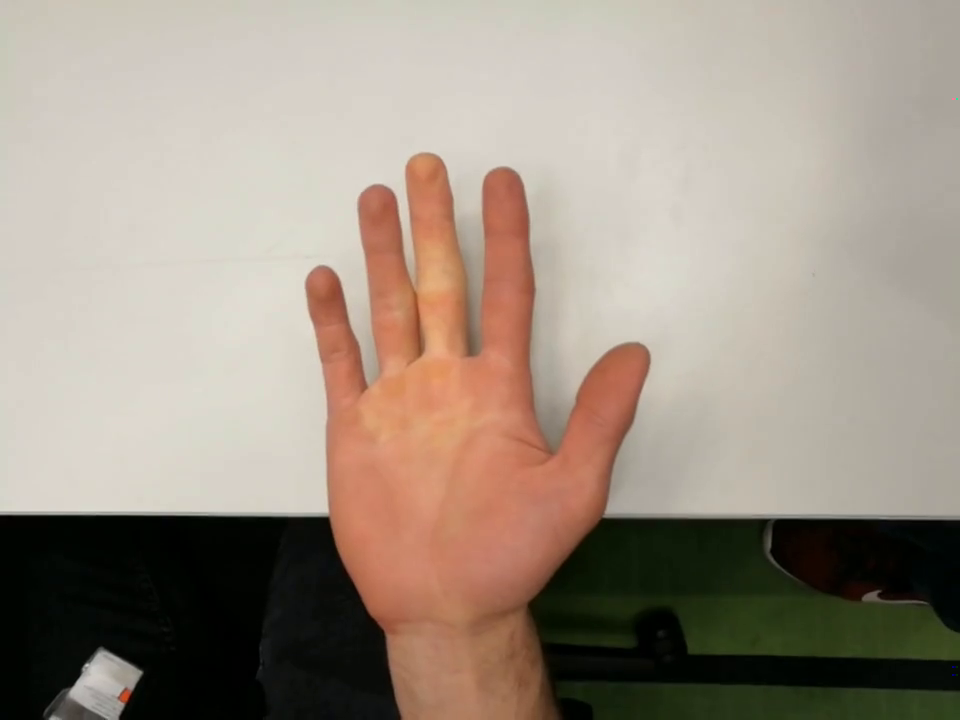
\includegraphics[width=100pt]{figures/flx_middle1}
  \caption{G4: Middle finger extension and flexion with the palm facing upwards}
  \end{subfigure}\par\medskip
  \begin{subfigure}[t]{0.5\linewidth}
  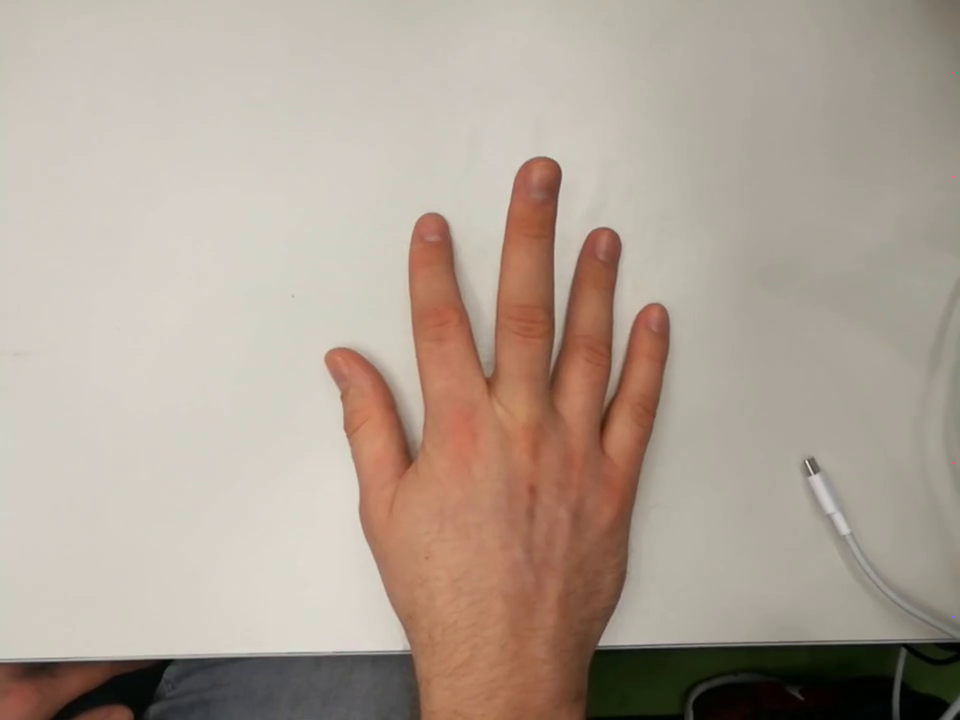
\includegraphics[width=100pt]{figures/ext_middle2}
  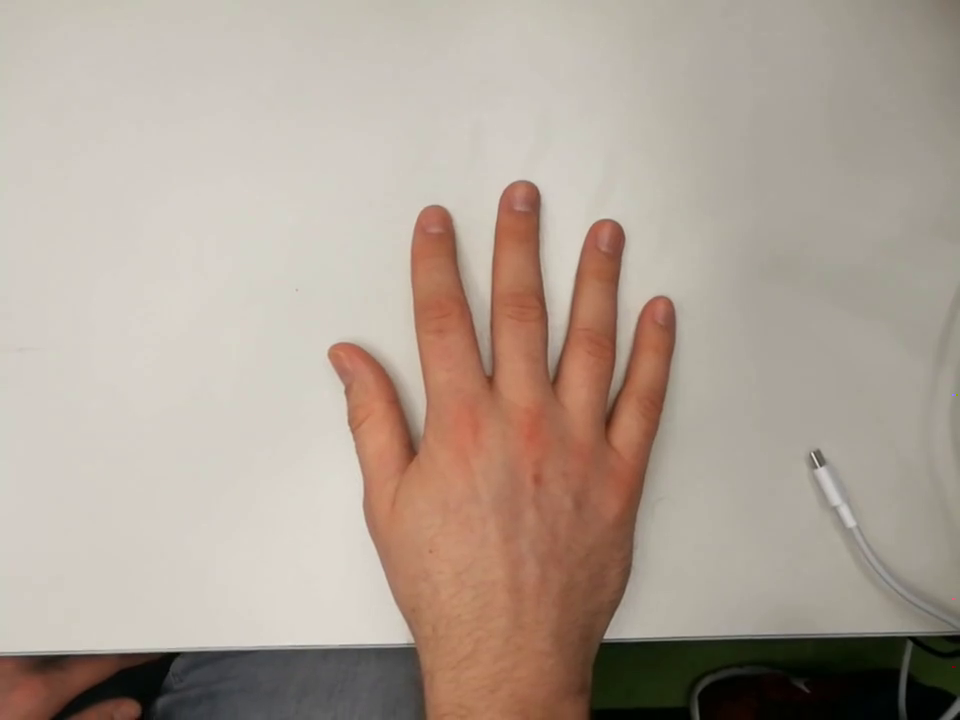
\includegraphics[width=100pt]{figures/flx_middle2}
  \caption{G5: Middle finger extension and flexion with the palm facing downwards}
  \end{subfigure}
  \hspace*{\fill}
  \begin{subfigure}[t]{0.5\linewidth}
  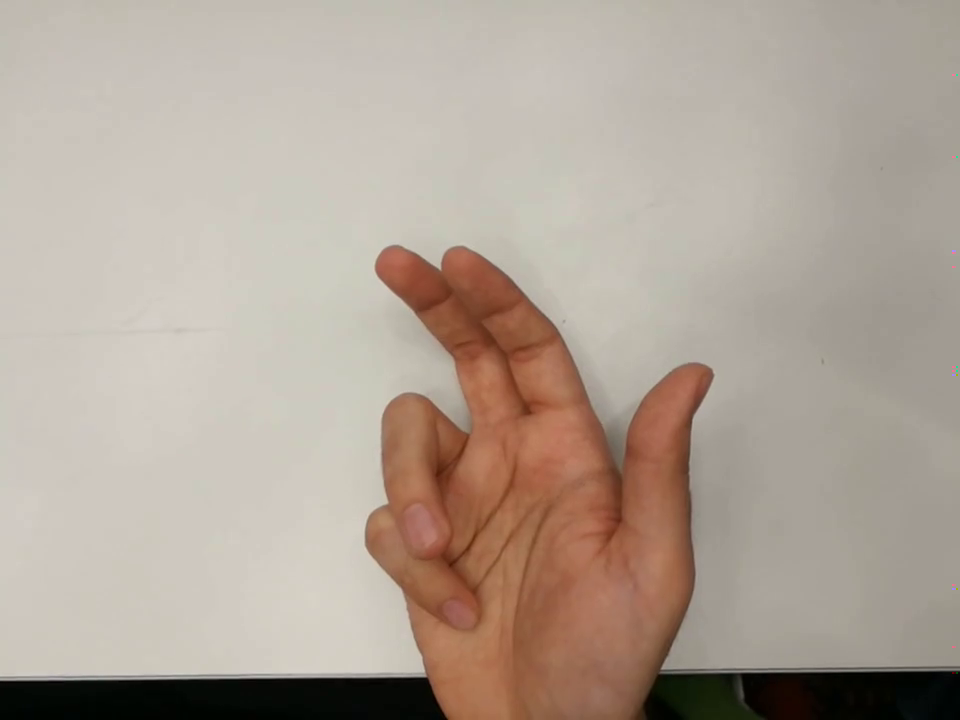
\includegraphics[width=100pt]{figures/ext_pinky1}
  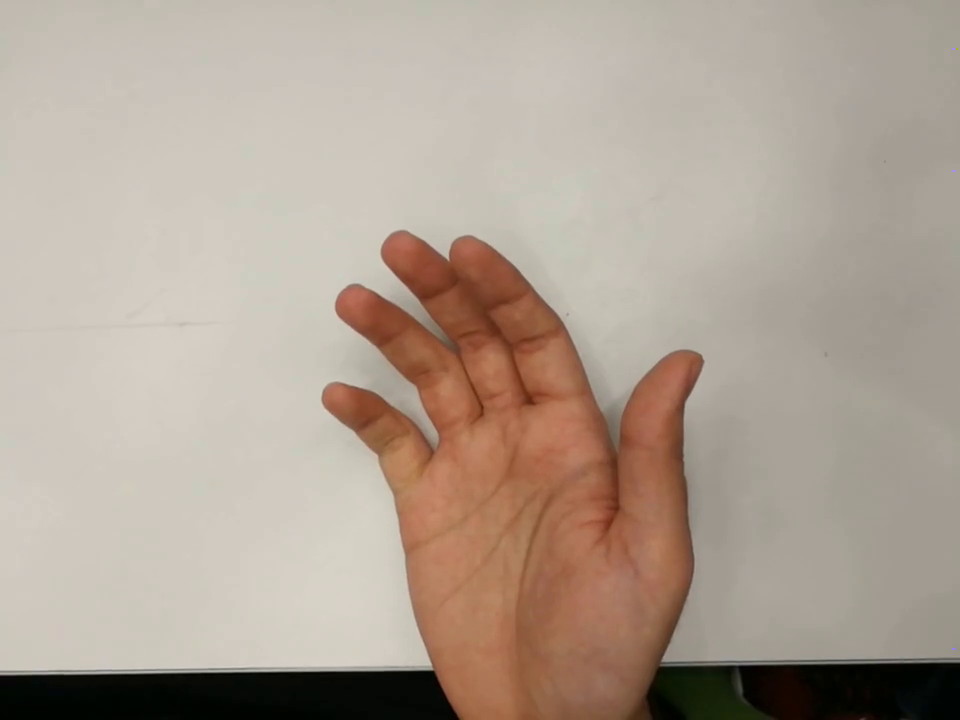
\includegraphics[width=100pt]{figures/flx_pinky1}
  \caption{G6: Pinky finger extension and flexion with the palm facing upwards}
  \end{subfigure}\par\medskip
  \begin{subfigure}[t]{0.5\linewidth}
  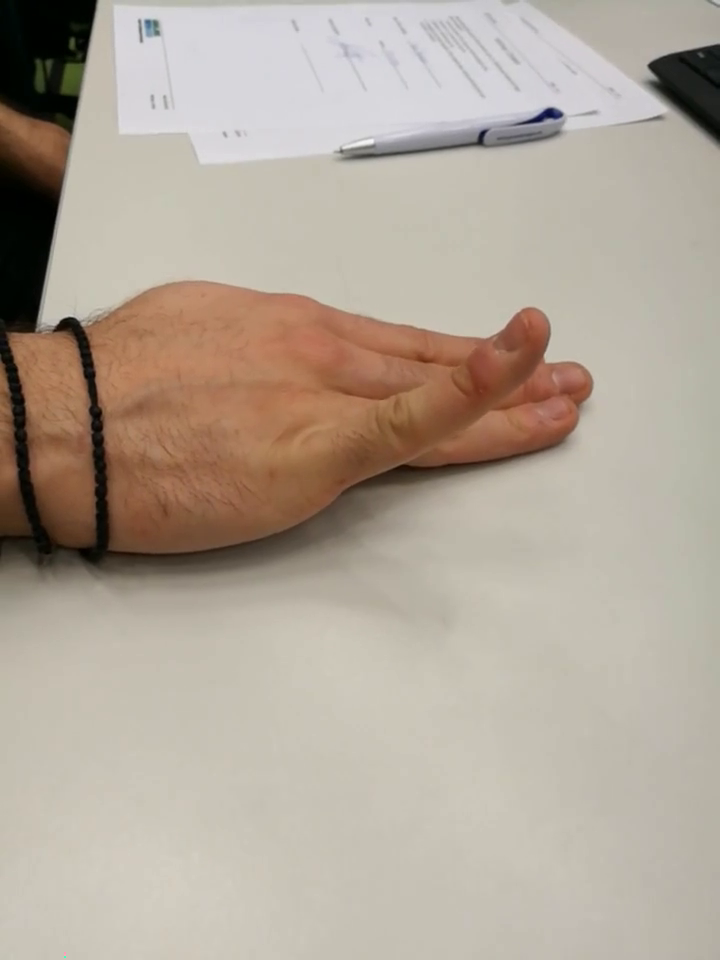
\includegraphics[width=100pt]{figures/ext_pinky2}
  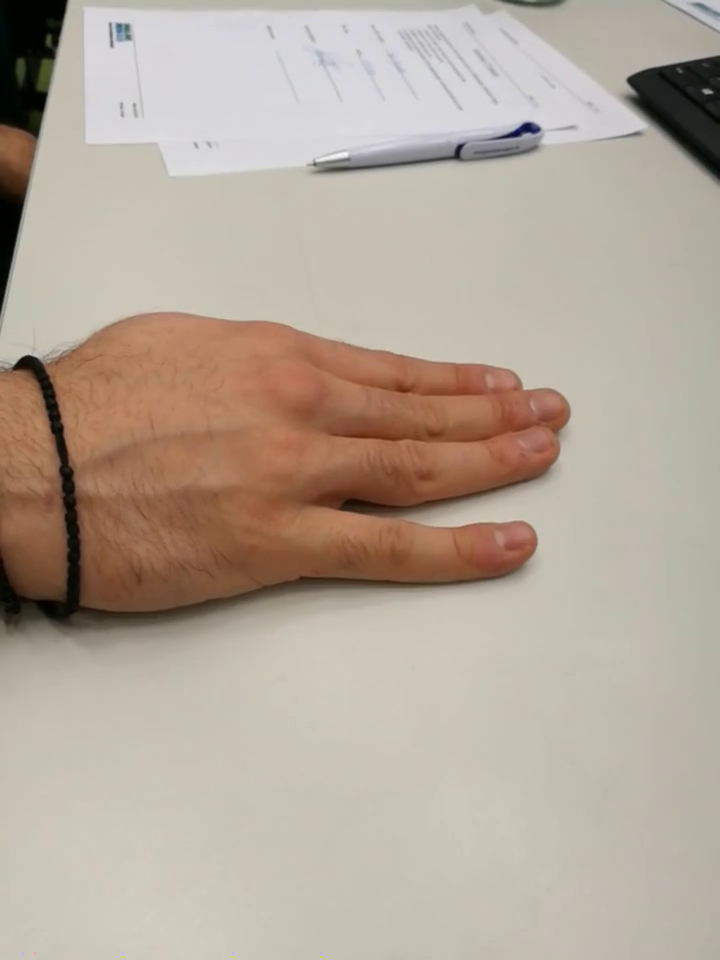
\includegraphics[width=100pt]{figures/flx_pinky2}
  \caption{G7: Pinky finger extension and flexion with the palm facing downwards}
  \end{subfigure}
  \hspace*{\fill}
  \begin{subfigure}[t]{0.5\linewidth}
  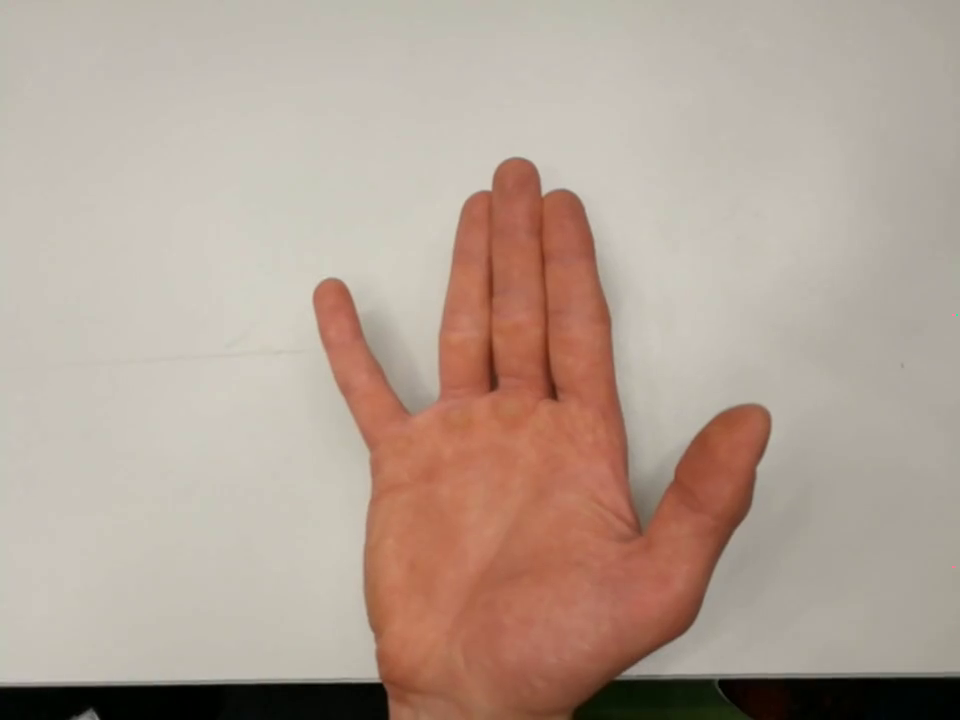
\includegraphics[width=100pt]{figures/ext_pinkytopair}
  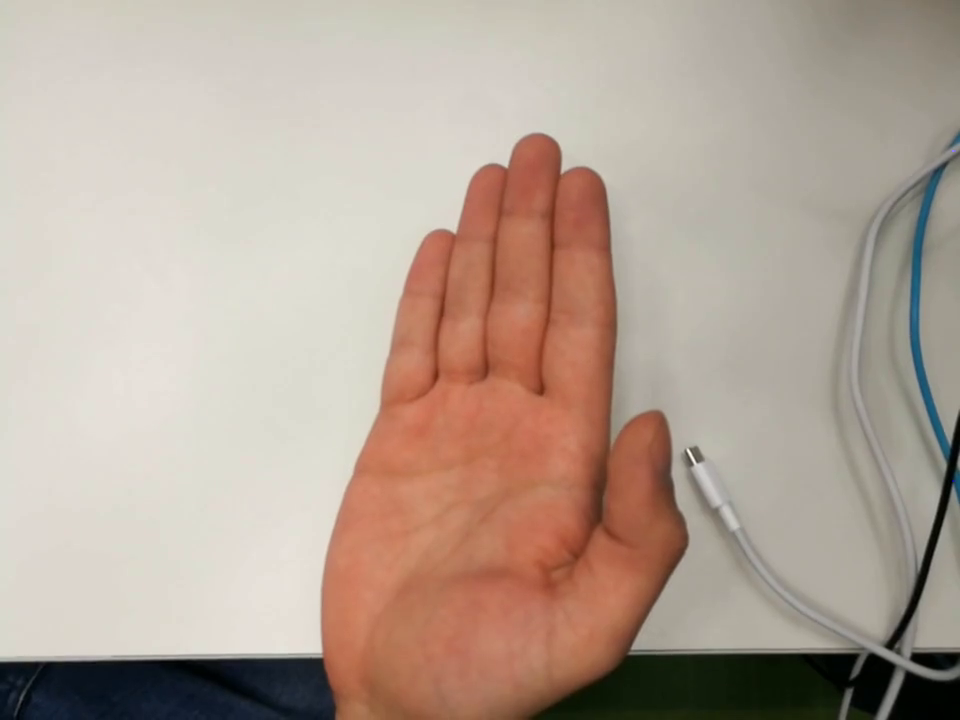
\includegraphics[width=100pt]{figures/flx_pinkytopair}
  \caption{G8: Moving pinky finger from and to pair (ring, middle, index)}
  \end{subfigure}\par\medskip
  \begin{subfigure}[t]{0.5\linewidth}
  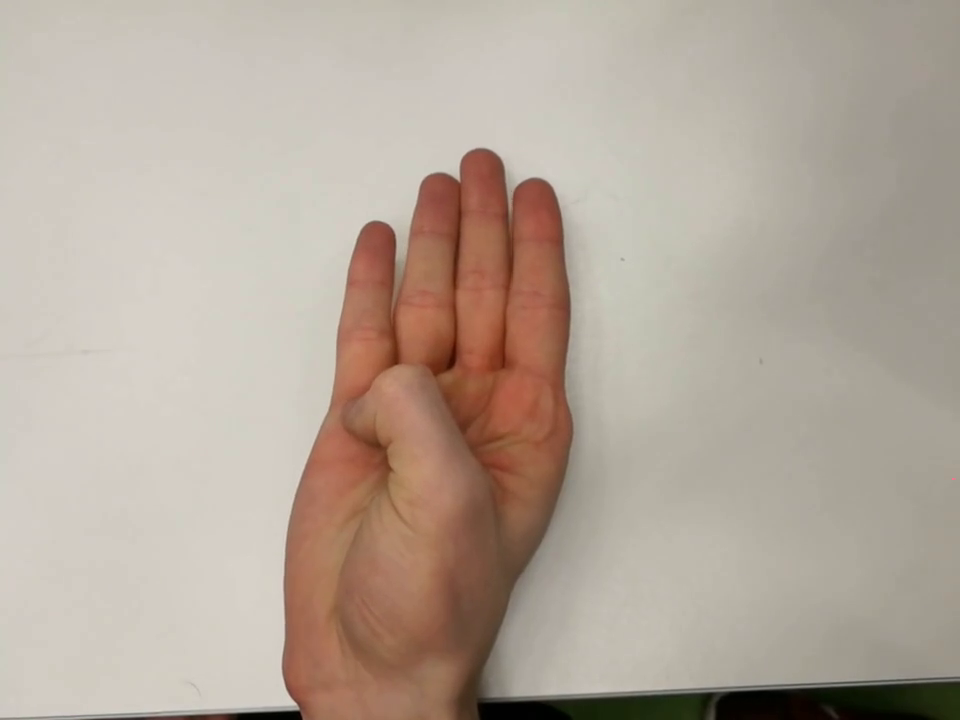
\includegraphics[width=100pt]{figures/ext_thumb1}
  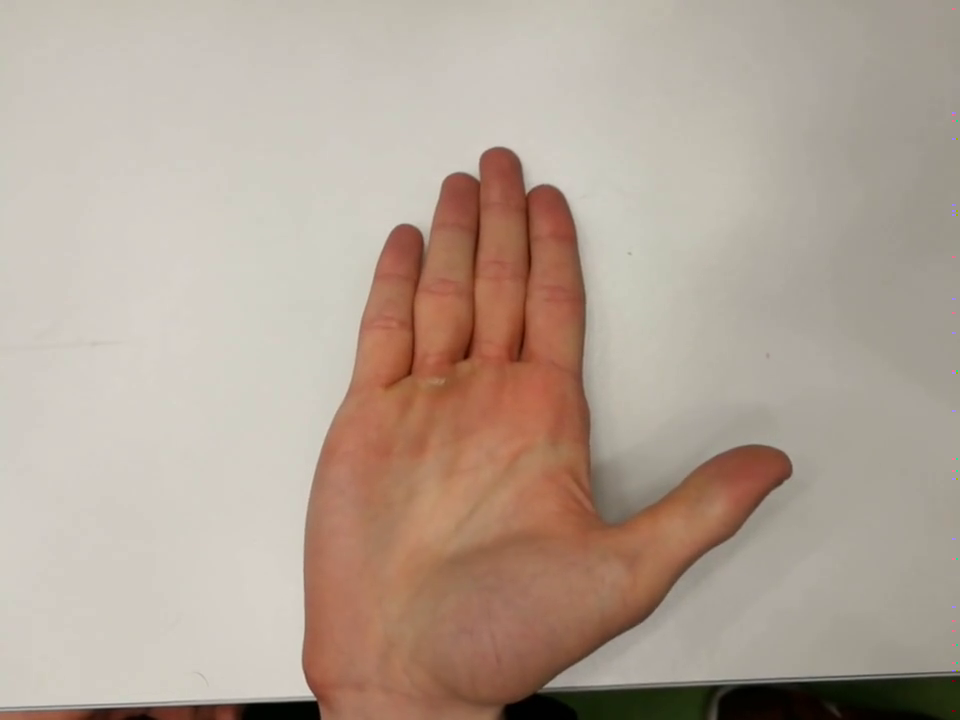
\includegraphics[width=100pt]{figures/flx_thumb1}
  \caption{G9: Thumb finger extension and flexion with the palm facing upwards}
  \end{subfigure}
  \hspace*{\fill}
  \begin{subfigure}[t]{0.5\linewidth}
  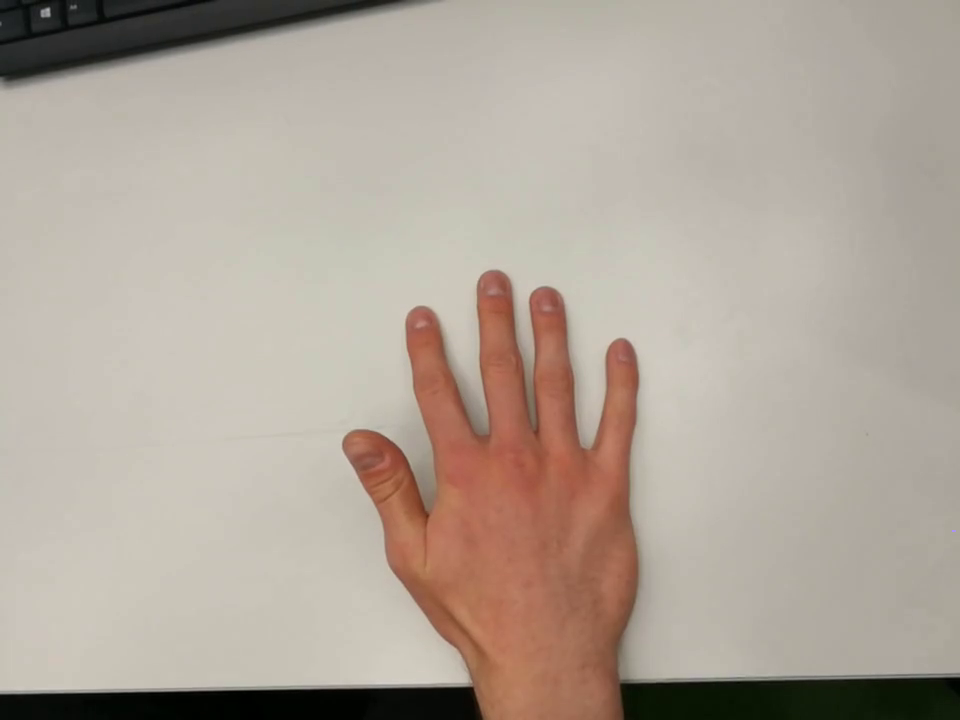
\includegraphics[width=100pt]{figures/ext_thumb2}
  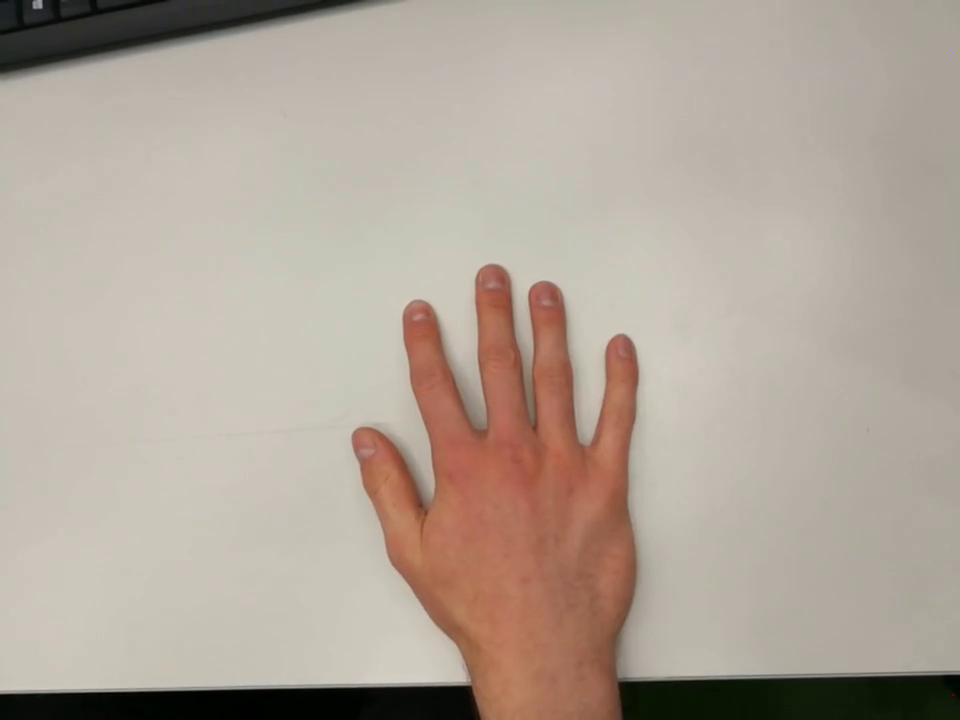
\includegraphics[width=100pt]{figures/flx_thumb2}
  \caption{G10: Thumb finger extension and flexion with the palm facing downwards}
  \end{subfigure}\par\medskip
\end{figure}
\begin{figure}
  \begin{subfigure}[t]{0.5\linewidth}
  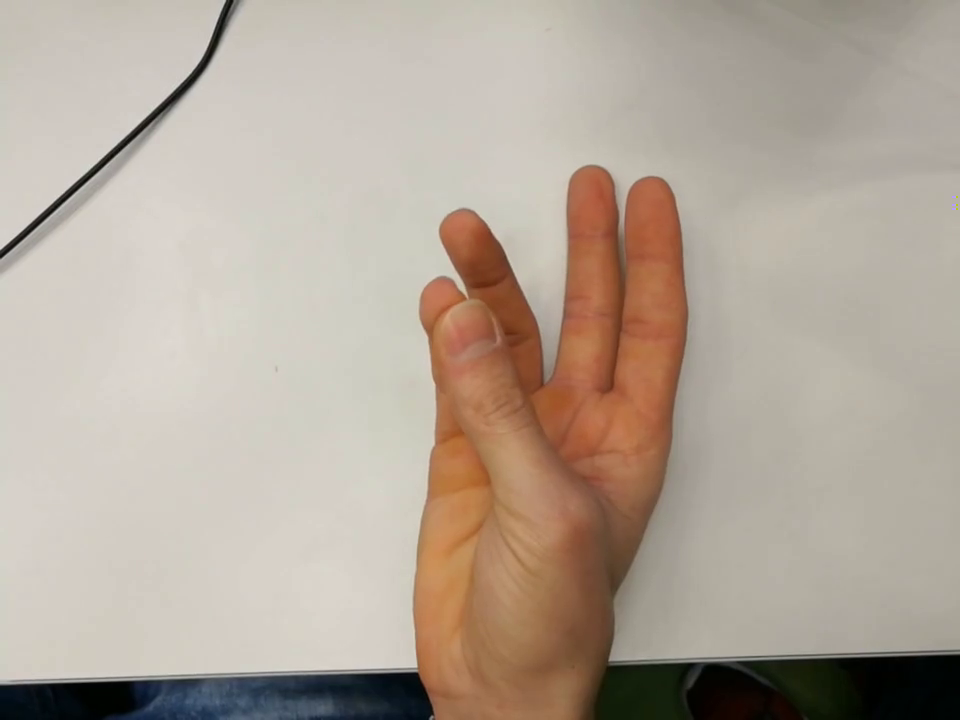
\includegraphics[width=100pt]{figures/ext_thumbtopinky}
  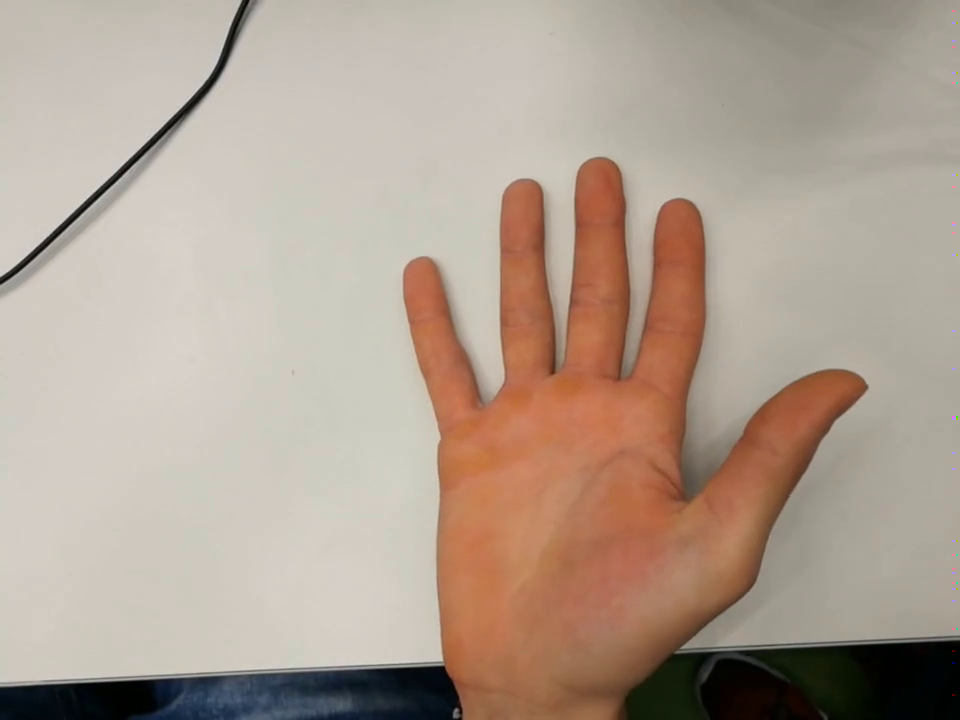
\includegraphics[width=100pt]{figures/flx_thumbtopinky}
  \caption{G11: Pairing and unpairing thumb with pinky}
  \end{subfigure}
  \hspace*{\fill}
  \begin{subfigure}[t]{0.5\linewidth}
  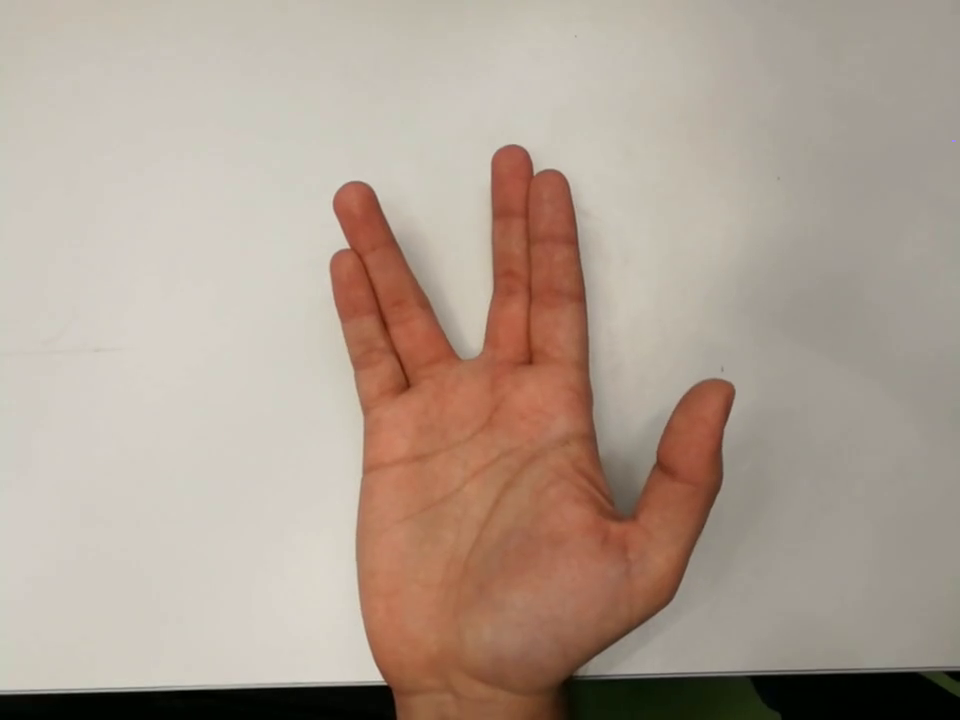
\includegraphics[width=100pt]{figures/ext_vulcan}
  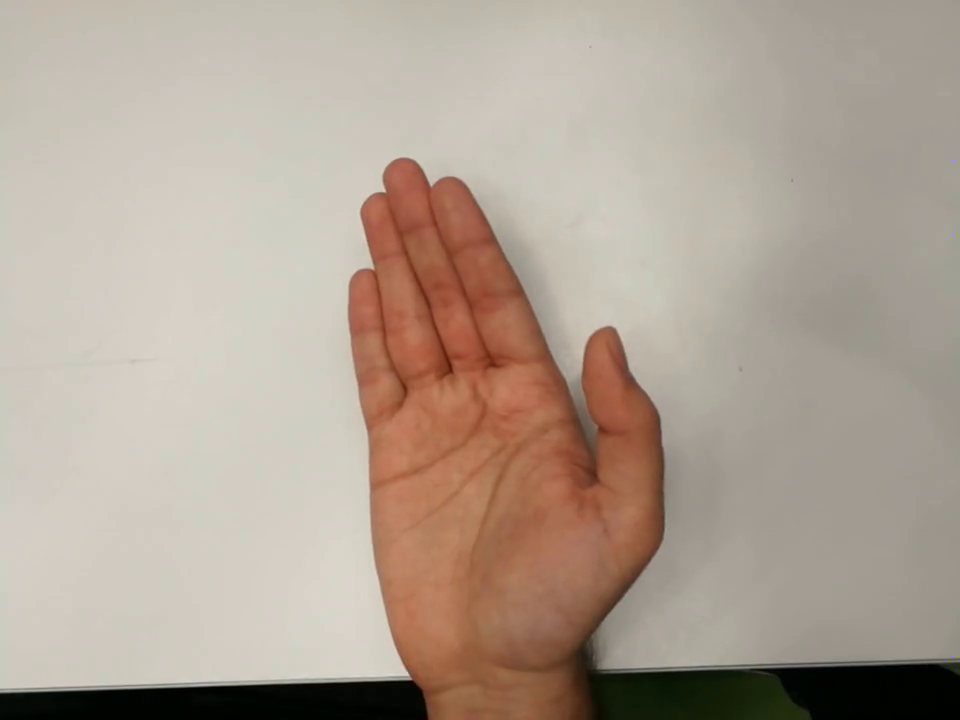
\includegraphics[width=100pt]{figures/flx_vulcan}
  \caption{G12: Pairing and unpairing pair1(index, middle) with pair2(ring, pinky)}
  \end{subfigure}\par\medskip 
  \begin{subfigure}[t]{0.5\linewidth}
  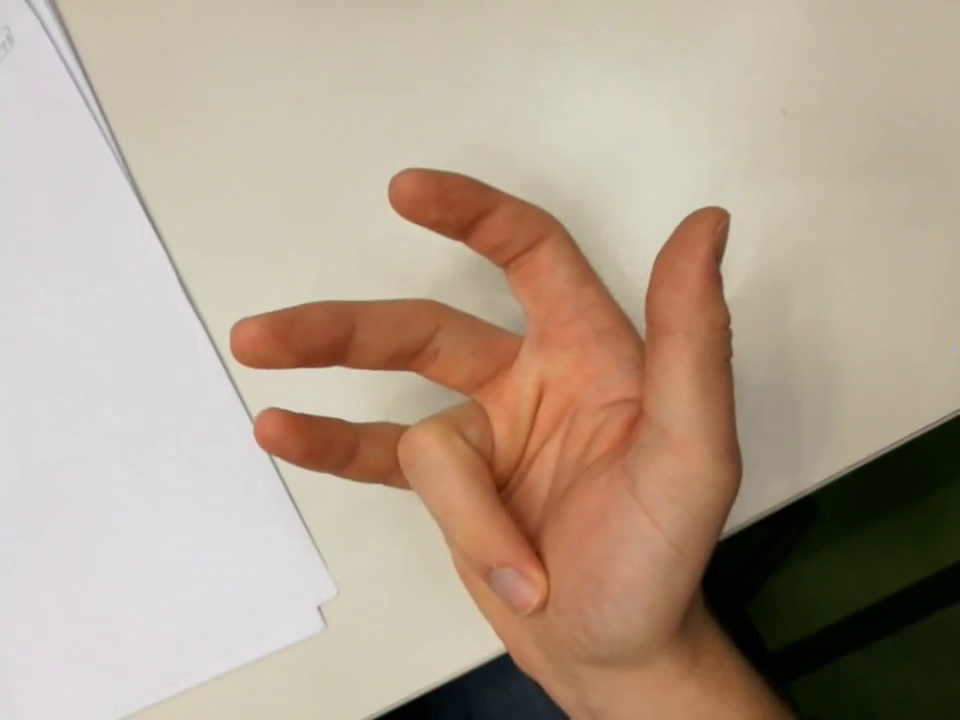
\includegraphics[width=100pt]{figures/ext_wedding1}
  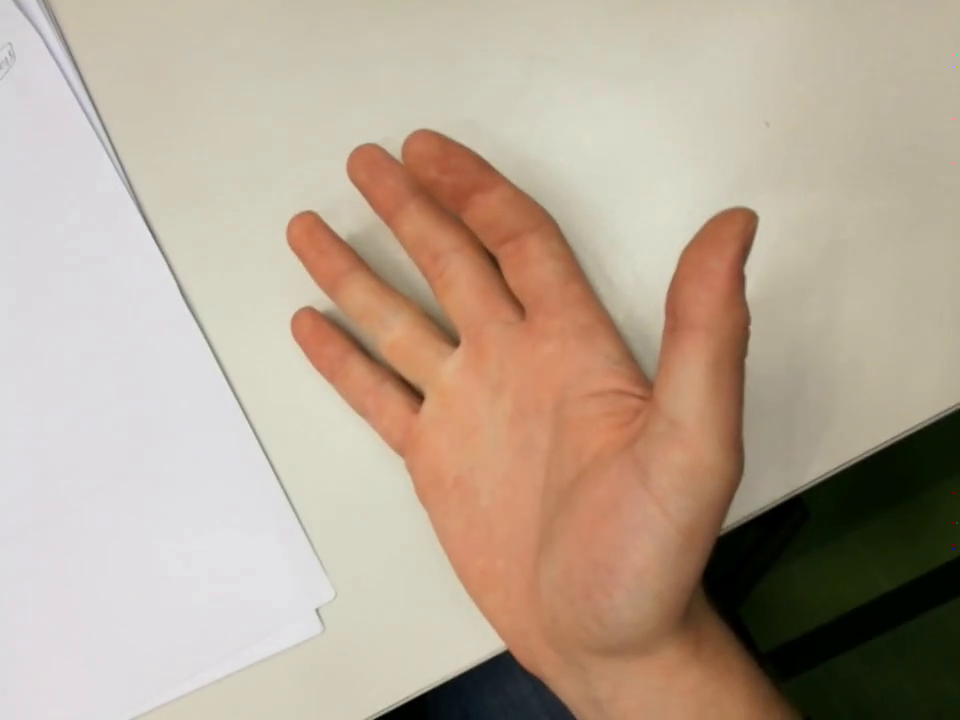
\includegraphics[width=100pt]{figures/flx_wedding1}
  \caption{G13: Rind finger extension and flexion with the palm facing upwards}
  \end{subfigure}
  \hspace*{\fill}
  \begin{subfigure}[t]{0.5\linewidth}
  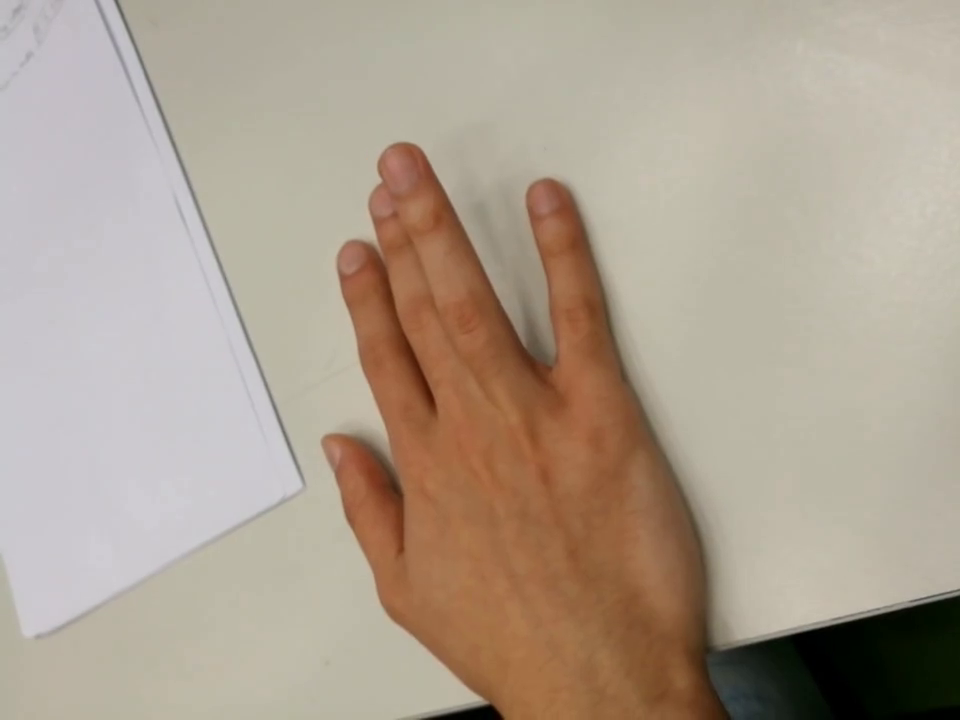
\includegraphics[width=100pt]{figures/ext_wedding2}
  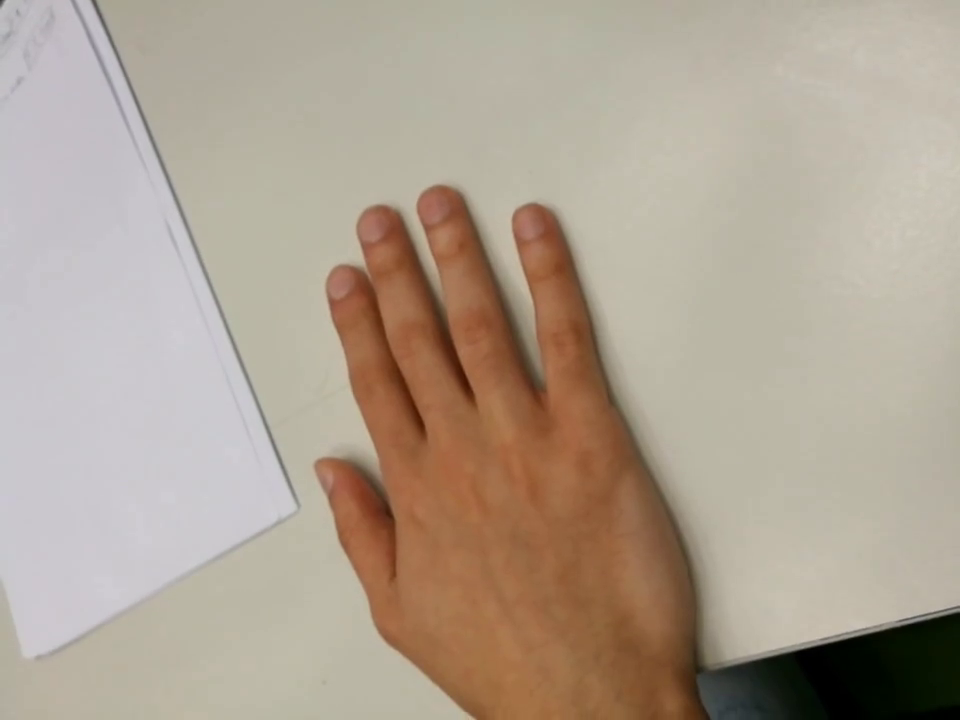
\includegraphics[width=100pt]{figures/flx_wedding2}
  \caption{G14: Ring finger extension and flexion with the palm facing downwards}
  \end{subfigure}\par\medskip
\caption{14 finger gestures from 21 different subjects were acquired using the Myo armband}
\end{figure}